\documentclass[pdflatex,sn-basic]{sn-jnl}

\usepackage{booktabs}
\usepackage{array}
\usepackage{tabularx}
\usepackage{longtable}
\usepackage{float}
\usepackage{amsmath,amssymb,amsfonts}
\usepackage{xcolor}
\usepackage{tikz}
\usetikzlibrary{arrows.meta,positioning,shapes.geometric,calc,patterns}

\newcolumntype{Y}{>{\raggedright\arraybackslash}X}
\newcolumntype{L}[1]{>{\raggedright\arraybackslash}p{#1}}
\newcommand{\codeid}[1]{\texttt{\detokenize{#1}}}
\newcommand{\pathid}[1]{\nolinkurl{#1}}
\newcommand{\rate}[2]{#1/#2}
\sloppy
\raggedbottom

\newcommand{\papertitle}{Measuring Dependency Hallucination in Generated Code: An End-to-End Validity Study}
\IfFileExists{submission_metadata_sqj.tex}{
  % SQJ identified-author metadata. Shiyong Xiong is the second author and corresponding author.
\author[1]{\fnm{Haonan} \sur{Wang}}
\author*[1]{\fnm{Shiyong} \sur{Xiong}}\email{xiongsy@cqupt.edu.cn}
\affil[1]{\orgdiv{School of Computer Science}, \orgname{Chongqing University of Posts and Telecommunications}, \orgaddress{\street{Xinke Building 10-09, Nan'an District}, \city{Chongqing}, \postcode{400065}, \country{China}}}
% Add ORCID identifiers if available, using the syntax supported by sn-jnl.

}{
  \author[1]{\fnm{Haonan} \sur{Wang}}
  \author*[1]{\fnm{Shiyong} \sur{Xiong}}\email{xiongsy@cqupt.edu.cn}
  \affil*[1]{\orgdiv{School of Computer Science}, \orgname{Chongqing University of Posts and Telecommunications}, \orgaddress{\street{Xinke Building 10-09, Chongqing University of Posts and Telecommunications, Nan'an District}, \city{Chongqing}, \postcode{400065}, \country{China}}}
}
\hypersetup{
  pdftitle={Measuring Dependency Hallucination in Generated Code: An End-to-End Validity Study},
  pdfauthor={Haonan Wang; Shiyong Xiong},
  pdfsubject={Measurement validity and external evaluation of dependency-hallucination signals in generated code},
  pdfkeywords={software quality, code generation, dependency hallucination, dependency analysis, buildability, measurement validity},
  hypertexnames=false
}

\begin{document}

\title[Measuring dependency hallucination]{\papertitle}
\abstract{Generated-code dependency signals are difficult to interpret unless extraction, evidence-based classification, and end-to-end detection are evaluated separately. We examine this measurement problem using a Python package-hallucination replication and Java import/dependency studies grounded in registries, project sources, platform resolution, human review, and bounded compiler probes. On 598 in-corpus Java candidates, post-extraction classification precision/recall are 0.971/0.653; a raw-response audit of 416 answers estimates end-to-end precision/recall at 0.971/0.210. In a frozen prospective evaluation of 200 answers from 30 new Java/Maven repositories, two annotators enumerate mentions with an F1 score of 0.499; 262 of 543 adjudicated mentions remain uncertain. The revised extractor (V2) raises end-to-end recall from 0.103 to 0.504, but precision is 0.319 (project-clustered 95\% confidence interval 0.069--0.619), failing the preregistered 0.90 precision gate. Only 2/30 external projects pass a nonzero-test baseline, so the planned engineering intervention stops before execution. The results identify extraction coverage, label uncertainty, and build eligibility as limits on software-quality claims. They support measurement and human-reviewed auditing, not a validated detector, autonomous dependency removal, functional correctness, or developer-practice effects.}
\keywords{software quality, measurement validity, code generation, dependency hallucination, dependency analysis, buildability}
\maketitle

\section{Introduction}

Large language models (LLMs) are now routinely used as programming assistants. They generate code snippets, explain APIs, recommend libraries, and produce dependency declarations that developers may copy into real projects. HumanEval made functional code generation measurable through executable unit tests.\citep{Chen2021Codex} MBPP broadened this style of evaluation with mostly basic Python programming tasks.\citep{Austin2021ProgramSynthesis} AlphaCode showed that large code models can compete on programming-contest style problems.\citep{Li2022AlphaCode} SWE-bench moved evaluation toward repository-level software issue resolution.\citep{Jimenez2024SWEbench} This convenience also creates a reliability problem: when a model confidently references a non-existent package, import path, method, class, or dependency coordinate, the result is not merely a wrong answer. It can waste debugging time, break builds, and in open package ecosystems create a supply-chain attack surface.

Recent work has made this risk concrete. Package hallucination research shows that code-generating LLMs can recommend non-existent packages and that such names may become exploitable if attackers register them in public package repositories.\citep{Spracklen2025} Empirical work on the npm ecosystem shows that dependency ecosystems can expose downstream projects to vulnerable or malicious packages.\citep{Zimmermann2019NPM} A broader review of open-source supply-chain attacks shows that dependency confusion and malicious package distribution are recurring risks.\citep{Ohm2020Backstabber} CloudAPIBench shows a related API-level failure mode: code models struggle with low-frequency cloud APIs, and documentation augmentation is not uniformly beneficial.\citep{Jain2024} MARIN studies API hallucination in practical projects and provides APIHulBench as a project-oriented benchmark.\citep{Chen2025MARIN} THINK reports that third-party-library API hallucinations can be reduced by knowledge injection and post-execution optimization.\citep{Liu2025THINK} HalluCode frames code hallucination beyond functional correctness through intent, consistency, and real-world-knowledge categories.\citep{Liu2024HalluCode} CodeHalu further shows that generated code can fail under execution, naming, mapping, resource, or logic checks.\citep{Tian2025CodeHalu}

Despite this progress, dependency hallucination remains under-specified from a software engineering perspective. Existing package-hallucination measurements primarily target package-name recommendations in Python and JavaScript. Existing API-hallucination mitigation methods often focus on retrieving documentation, grounding project APIs, or constraining generation. These lines are complementary, but they leave a practical gap: in real generated code, dependencies appear through multiple surfaces, including package recommendations, install commands, Maven coordinates, Gradle declarations, Java import statements, and project-looking namespace paths. A robust measurement pipeline should therefore ask not only whether a string exists in a registry, but also whether it is a standard-library token, a module path, a project-local symbol, a valid external dependency, or a suspicious dependency mention likely to break a build.

This paper treats dependency-hallucination signals as a measurement problem with implications for dependency integrity and buildability, not as a complete measure of software quality. We operationalize three distinct outcomes: mention extraction, evidence-grounded validity classification, and bounded compilation evidence. These are proxies for dependency integrity and buildability; they do not measure functional correctness, maintainability, or developer productivity. We reproduce the Package Hallucination protocol locally on Python and report rule-stratified package signals without treating them as human-validated labels. For Java, we separate extraction, classification, and end-to-end detection using Maven registry evidence, project-source indexes, platform resolution, and human audits. Dependency-seeking and masked-import protocols examine dependency evidence under explicit prompting; compiler probes provide bounded buildability evidence, not functional or test-quality outcomes. Repair and removal experiments are diagnostic baselines only. The prospective engineering intervention does not reach its preregistered eligibility threshold and is not used to claim a practice effect.

This study makes four contributions to software-quality measurement:

\begin{enumerate}
  \item An explicit measurement decomposition that distinguishes candidate extraction, conditional validity classification, and end-to-end detection across package and import surfaces.
  \item A human-audited Java characterization showing that high conditional precision can coexist with low extraction coverage and low end-to-end recall; these metrics are treated as in-corpus characterization rather than independent detector validation.
  \item A frozen, project-disjoint evaluation of V1/V2 that quantifies the recall--precision trade-off and exposes substantial mention-enumeration and label uncertainty.
  \item Bounded compiler-facing evidence and a preregistered engineering stop that define what the current data can and cannot establish about buildability and software-quality effects.
\end{enumerate}

Fig.~\ref{fig:pipeline} summarizes the complete measurement pipeline.

\begin{figure}[htbp]
\centering
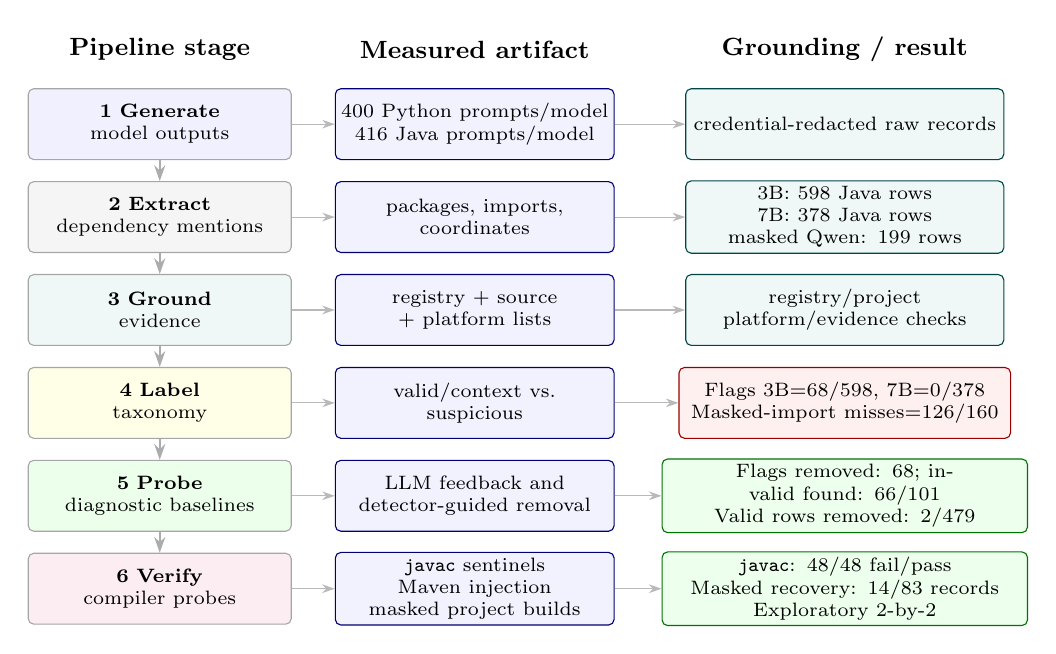
\begin{tikzpicture}[
  font=\scriptsize,
  header/.style={font=\bfseries\small, align=center},
  stage/.style={draw=gray!70, rounded corners=2pt, align=center, text width=32mm, minimum height=9mm, inner sep=2pt, fill=gray!7},
  artifact/.style={draw=blue!45!black, rounded corners=2pt, align=center, text width=34mm, minimum height=9mm, inner sep=2pt, fill=blue!5},
  evidence/.style={draw=teal!55!black, rounded corners=2pt, align=center, text width=39mm, minimum height=9mm, inner sep=2pt, fill=teal!6},
  impact/.style={draw=green!45!black, rounded corners=2pt, align=center, text width=39mm, minimum height=9mm, inner sep=2pt, fill=green!7},
  risk/.style={draw=red!60!black, rounded corners=2pt, align=center, text width=40mm, minimum height=9mm, inner sep=3pt, fill=red!6},
  arrow/.style={-{Stealth[length=2mm,width=1.4mm]}, thick, draw=gray!65},
  link/.style={-{Stealth[length=1.6mm,width=1.1mm]}, draw=gray!55}
]
\node[header] at (0,0.95) {Pipeline stage};
\node[header] at (4.0,0.95) {Measured artifact};
\node[header] at (8.7,0.95) {Grounding / result};

\node[stage, fill=blue!6] (s1) at (0,0) {\textbf{1 Generate}\\model outputs};
\node[artifact] (a1) at (4.0,0) {400 Python prompts/model\\416 Java prompts/model};
\node[evidence] (e1) at (8.7,0) {credential-redacted raw records};

\node[stage, fill=gray!8] (s2) at (0,-1.18) {\textbf{2 Extract}\\dependency mentions};
\node[artifact] (a2) at (4.0,-1.18) {packages, imports,\\coordinates};
\node[evidence] (e2) at (8.7,-1.18) {3B: 598 Java rows\\7B: 378 Java rows\\masked Qwen: 199 rows};

\node[stage, fill=teal!6] (s3) at (0,-2.36) {\textbf{3 Ground}\\evidence};
\node[artifact] (a3) at (4.0,-2.36) {registry + source\\+ platform lists};
\node[evidence] (e3) at (8.7,-2.36) {registry/project\\platform/evidence checks};

\node[stage, fill=yellow!10] (s4) at (0,-3.54) {\textbf{4 Label}\\taxonomy};
\node[artifact] (a4) at (4.0,-3.54) {valid/context vs.\\suspicious};
\node[risk] (e4) at (8.7,-3.54) {Flags 3B=68/598, 7B=0/378\\Masked-import misses=126/160};

\node[stage, fill=green!8] (s5) at (0,-4.72) {\textbf{5 Probe}\\diagnostic baselines};
\node[artifact] (a5) at (4.0,-4.72) {LLM feedback and\\detector-guided removal};
\node[impact, text width=45mm] (e5) at (8.7,-4.72) {Flags removed: 68; invalid found: 66/101\\Valid rows removed: 2/479};

\node[stage, fill=purple!7] (s6) at (0,-5.90) {\textbf{6 Verify}\\compiler probes};
\node[artifact] (a6) at (4.0,-5.90) {\codeid{javac} sentinels\\Maven injection\\masked project builds};
\node[impact, text width=45mm] (e6) at (8.7,-5.90) {\codeid{javac}: 48/48 fail/pass\\Masked recovery: 14/83 records\\Exploratory 2-by-2};

\foreach \from/\to in {s1/s2,s2/s3,s3/s4,s4/s5,s5/s6} {
  \draw[arrow] (\from.south) -- (\to.north);
}
\foreach \from/\to in {s1/a1,a1/e1,s2/a2,a2/e2,s3/a3,a3/e3,s4/a4,a4/e4,s5/a5,a5/e5,s6/a6,a6/e6} {
  \draw[link] (\from.east) -- (\to.west);
}
\end{tikzpicture}
\caption{Registry-, project-, evidence-, and compilation-aware dependency-validity measurement pipeline. The right column reports measured evidence and bounded outcomes, not full-code correctness}
\label{fig:pipeline}
\end{figure}

\section{Related Work}

\subsection{Code Hallucination Taxonomies and Benchmarks}

Recent software engineering research has begun to define code-specific hallucination categories. HalluCode studies hallucinations in LLM-generated code beyond functional correctness and provides a taxonomy that includes intent deviation, internal inconsistency, and misalignment with real-world knowledge.\citep{Liu2024HalluCode} CodeHalu evaluates hallucinations through execution-based verification and categorizes failures into mapping, naming, resource, and logic hallucinations.\citep{Tian2025CodeHalu} These works motivate our distinction between raw detector output and grounded dependency labels: a generated identifier may look plausible while being unsupported by a package registry, project source tree, or build system.

\subsection{Package and Library Hallucinations}

The closest baseline is the USENIX Security 2025 Package Hallucination study.\citep{Spracklen2025} Its artifact measures package hallucination by generating code, querying models for required packages, and comparing package names against registries. Importing Phantoms complements this security framing by measuring package hallucination vulnerabilities across programming languages and showing that hallucination rates vary with model choice, language, model size, and task specificity.\citep{Krishna2025Phantoms} Our Python replication preserves the Package Hallucination protocol for comparability. We extend it with deterministic post-labeling strata because many apparent package hallucinations in a local pilot are module paths, standard-library names, or ecosystem aliases rather than missing PyPI package names.

Recent library-hallucination work grounded in realistic developer queries further shows that prompt variation, misspellings, and fabricated library names can increase invalid library and member references.\citep{Twist2025LibHallu} This supports our broader dependency view: users and models express dependencies through package names, imports, natural-language library references, and dependency declarations, so detector design should cover more than one textual surface.

\subsection{API Hallucination and Project-Specific Grounding}

API hallucination is closely related to dependency hallucination because a fabricated import path or class name can be viewed as a dependency-level symptom of the same grounding failure. CloudAPIBench evaluates code LLM hallucinations for cloud APIs and shows that low-frequency APIs remain difficult; documentation-augmented generation helps, but poor retrieval can also harm high-frequency API generation.\citep{Jain2024} De-Hallucinator grounds code generation by retrieving project-specific API references using iterative model feedback.\citep{Eghbali2024} These results motivate our project-source grounding: not every valid dependency mention exists in a public registry, and not every plausible project namespace exists in the target project.

MARIN, accepted to the FSE 2025 Industry Track, directly targets API hallucination in practical projects and introduces APIHulBench, Micro Hallucination Number, and Macro Hallucination Rate.\citep{Chen2025MARIN} THINK, accepted at SANER 2025, uses knowledge injection for third-party-library API hallucinations and combines pre-execution retrieval enhancement with post-execution optimization.\citep{Liu2025THINK} Compared with these methods, our route is narrower but more artifact-oriented: we focus on transparent extraction, dependency/import taxonomy labels, deterministic sanitization, and build-level evidence for Java dependency mentions.

Recent API mapping evaluation also reports high hallucinated API rates under low-resource and cross-language conditions, with retrieval-augmented generation reducing but not eliminating the issue.\citep{Han2026APIMapping} This supports our methodological stance that model scale, retrieval, and grounding must be measured empirically rather than assumed to solve the problem.

\subsection{Code Models, Retrieval, and Grounding}

Code-specialized LLMs are trained and evaluated over increasingly large code corpora and benchmarks. CodeGen demonstrates the effectiveness of large autoregressive code models for multi-turn program synthesis.\citep{Nijkamp2023CodeGen} Code Llama extends this line with open foundation models specialized for code generation and infilling.\citep{Roziere2024CodeLlama} The Stack documents the scale and governance issues involved in assembling permissively licensed code corpora.\citep{Kocetkov2023Stack} These developments make dependency hallucination more consequential: model outputs can look idiomatic because they are shaped by real code distributions, even when a particular dependency name or project namespace is fabricated.

Dense passage retrieval provides a reusable mechanism for grounding generation in retrieved evidence.\citep{Karpukhin2020DPR} Retrieval-augmented generation connects retrieval with sequence generation for knowledge-intensive tasks.\citep{Lewis2020RAG} Retrieval-augmented code generation extends this idea to software artifacts by conditioning generation on related code or summaries.\citep{Parvez2021RetrievalCode} Our work is complementary: instead of proposing a new retriever, we use registry, project-source, and build evidence to evaluate and sanitize dependency mentions after generation.

\subsection{Dependency Management and Build Practice}

Dependency validity is also a long-standing software-engineering concern outside LLM research. Static dependency analysis can be inaccurate when language features and analysis configurations are not represented faithfully, which motivates reporting evidence sources and classification boundaries.\citep{Pruijt2017DependencyAccuracy} Component release management treats dependency versions, configurations, and inter-component constraints as coordinated release artifacts rather than isolated names.\citep{VanDerHoek2003ReleaseManagement} Dependency solving has likewise been formulated as a distinct problem in component evolution management, where selecting compatible versions is separate from identifying a component.\citep{Abate2012DependencySolving} We connect these strands to our setting more narrowly: the Java audit is a dependency-analysis and component-evolution measurement problem at the generated-mention boundary. Registry lookup establishes ecosystem existence; project structure and platform resolution establish context; compiler probes test whether the resolved choice is actionable in a build. This positioning distinguishes our evidence-source ablation from work on release planning or dependency solvers, while explaining why a single registry check is insufficient.

Table~\ref{tab:related-comparison} positions the closest related work.

\begin{table}[htbp]
\caption{Positioning against closely related hallucination studies.}
\footnotesize
\setlength{\tabcolsep}{3pt}
\begin{tabularx}{\linewidth}{@{}L{22mm}L{31mm}L{38mm}Y@{}}
\toprule
Study & Main surface & Grounding or validation & Difference from this study \\
\midrule
Package study\citep{Spracklen2025} & Package names & Public package registries & We reproduce the package-check setting and add rule-stratified categories plus Java import/compilation evidence. \\
Cloud docs\citep{Jain2024} & Cloud API code & API documentation retrieval & We validate generated dependency/import mentions after generation rather than testing documentation-augmented prompting. \\
MARIN\citep{Chen2025MARIN} & Project API calls on APIHulBench & Hierarchical project dependencies; MaHR/MiHN & We use APIHulBench prompts but study import/dependency validity instead of exact API-call completion. \\
THINK\citep{Liu2025THINK} & Third-party APIs & Knowledge injection and post-execution optimization & We provide an auditable registry/project sanitizer and compiler-facing probes rather than an LLM knowledge-injection pipeline. \\
This study & Python packages; Java imports and dependencies & Registry, project-source, human-audit, and build/import probes & We combine a full rule-based sweep with a completed two-annotator audit and compiler-facing evidence. \\
\bottomrule
\end{tabularx}
\label{tab:related-comparison}
\end{table}

\section{Methodology}

\subsection{Research Questions}

Table~\ref{tab:research-questions} lists the three research questions.

\begin{table}[htbp]
\caption{Research questions.}
\label{tab:research-questions}
\begin{tabularx}{\linewidth}{@{}lY@{}}
\toprule
RQ & Question \\
\midrule
RQ1 & How do extraction, conditional classification, and end-to-end evaluation shape dependency-hallucination measurements across the Python package replication and Java import/dependency studies? \\
RQ2 & How do frozen V1/V2 pipelines perform on an independently annotated, project-disjoint Java corpus, and how sensitive are the estimates to mention and label uncertainty? \\
RQ3 & What bounded buildability evidence is available from the compiler and sanitizer probes, and what software-quality or practice-effect claims remain unsupported? \\
\bottomrule
\end{tabularx}
\end{table}

\par

\textbf{Scope and uncertainty.} The unit of analysis is dependency/import validity, not full functional correctness of generated programs. A sanitized completion may still be semantically incomplete or logically wrong. We therefore interpret sanitization as a transparent detector-flagged import-removal baseline and compiler probes as bounded evidence about import validity, injected-import impact, or test-compile-valid import recovery. The full 3B Java sweep is rule-based before audit, and the candidate-row audit provides human validation over all 598 \emph{extracted} rows. Precision, recall, and F1 are post-extraction validity-classification metrics on 580 rows with final valid/invalid labels; 15 malformed rows and 3 uncertain rows are excluded and reported separately. A separate raw-response audit covers all 416 answers and 1,026 adjudicated mentions; its extractor and end-to-end metrics are mention-level, descriptive, and project-clustered over 97 projects. Classification intervals use 10,000 project-clustered percentile bootstrap replicates with \codeid{project_path} as the resampling unit and seed 20260804; the raw-response audit uses seed 20260814. Candidate-row rates and compiler-pair proportions are descriptive because rows and targets are nested. The prospective evaluation contains 200 answers from 30 fixed-commit repositories and uses 10,000 project-clustered bootstrap replicates with seed 20260818. Its two annotators disagree materially on mention enumeration; uncertain adjudications are therefore excluded in the primary analysis and counted as positive and negative in separate sensitivity analyses. Prompt-level Java analyses and masked compilation analyses use their separately recorded project-clustered seeds and offsets.

\subsection{Artifacts and Datasets}

The Python replication uses the official Package Hallucination artifact and its four Python prompt families: \codeid{LLM_LY}, \codeid{LLM_AT}, \codeid{SO_LY}, and \codeid{SO_AT}. We sample 100 prompts from each family, giving 400 prompts per model. Each prompt is evaluated under two package-query modes. Q1 asks which packages are required to run the model-generated code. Q2 asks which packages are useful for solving the original programming prompt.

The Java extension uses five disjoint APIHulBench-derived Java prompt windows. The first three windows contain 100 prompts each, with 50 prompts from the functional split and 50 prompts from the method-level split. The fourth tail window starts at offset 150 and contains 95 prompts because the method-level split contributes 45 remaining records at that offset. The final F-only tail window starts at offset 200 and contains the remaining 21 functional-split records. The Java experiment therefore covers all 416 local APIHulBench F/M prompts. We run this full prompt set with Qwen2.5-Coder-3B-Instruct for the primary Java detector, audit, repair, sanitization, and compiler-probe results, and with Qwen2.5-Coder-7B-Instruct as a same-prompt detection control. We also run a 7B dependency-seeking stress prompt over the same 416 records; this prompt asks for an explicit dependency manifest but still permits the answer \codeid{No external dependency}. To strengthen the 7B stress denominator, we construct a dependency-critical masked-import set from the same 416 prompts. A record is eligible only when the source file exists, Maven or Gradle context exists, a source-indexed external dependency import appears in the current file prefix, and that import's simple name is referenced in the incomplete fragment. The strict main/test set contains 117 prompts and 160 hidden external imports after excluding custom/unknown source-set records and generated-source imports. The hidden imports remain in metadata for evaluation but are removed from the rendered prompt.

The masked-import selection flow is recorded as 416 local F/M records, 412 records with source files, 411 with source and build context, 209 with external dependency-import context, 121 where an external import is used in the incomplete fragment, 120 dependency-critical seeds, and 117 strict main/test prompts after exclusions. These 117 prompts span 60 projects and 85 build-context groups. The 160 hidden targets contain 85 unique fully qualified imports, with 75 repeated target instances and a maximum reuse of 19 for a single import. Exact hidden FQNs are not present in the rendered prompts. Because hidden-import targets are nested within records and projects, target-level proportions are interpreted with project-clustered uncertainty rather than as 160 independent observations.

\subsection{Models and Decoding}

The controlled Python comparison uses Qwen2.5-Coder-3B-Instruct and Qwen2.5-Coder-7B-Instruct, both in 4-bit local inference with deterministic decoding and 400 prompts.\citep{Hui2024Qwen25Coder} For brevity, subsequent compact labels use Qwen-3B and Qwen-7B for these two models. The primary Java extension uses Qwen-3B 4-bit; the same-prompt Java control uses Qwen-7B 4-bit with the same deterministic decoding and 384-token generation cap. The Qwen-7B dependency-seeking and dependency-critical masked-import stress runs use deterministic decoding with a 512-token cap so the model can emit both code and dependency manifest rows. A DeepSeek-Coder-6.7B-Instruct 4-bit run on the same 117 masked prompts is retained only as an appendix format-sensitivity experiment.\citep{Guo2024DeepSeekCoder} It uses a 1024-token cap, a tokenizer-file backend, no system message, and offline-only coordinate validation. These differences preclude a model-quality comparison. The appendix therefore reports observed manifest-format compliance, output length, and post-hoc ceiling proxies, and does not use DeepSeek to support the main model result. No full-precision counterpart is evaluated for any local model, so model-size observations cannot isolate parameter scale from checkpoint-specific quantization interactions. The LLM registry-feedback repair experiment is run on the first 3B Java window, on the Qwen-7B dependency-seeking targets, and on the 4 Qwen-7B detector-evidence records from the masked-import run. Deterministic sanitization and import-only compiler probing are run on all five 3B Java windows, and deterministic dependency sanitization is run on both Qwen-7B stress outputs. For the original Qwen-7B Java control, the enhanced detector flags no suspicious import rows, so that protocol contributes a zero-target, zero-edit sanitizer outcome rather than a repair-effect denominator.

\subsection{Use of Generative AI Tools}

GitHub Copilot was used to search GitHub for papers related to this study and to organize and summarize the retrieved literature. OpenAI Codex assisted with developing the study framework, experimental design, and manuscript drafting. Neither tool was used to generate the original model responses or annotator labels. Both authors reviewed the AI-assisted changes; Haonan Wang accepts responsibility for the reported implementation and analysis, and Shiyong Xiong accepts overall responsibility for the final manuscript.

\subsection{Python Package Hallucination Measurement}

For Python, we preserve comparability with the official detector by reporting raw registry-check rates. We then report artifact-filtered rates and deterministic rule-stratified registry-missing rates. The post-labeling rules assign each detector-positive mention to one of five categories: registry-missing candidate, artifact or placeholder noise, standard-library or builtin token, package-module path token, and alias or ecosystem package token. These categories are not independently annotated human truth and must not be interpreted as equivalent to the two-annotator Java audit.

To avoid relying only on mention denominators, we pair the same 400 prompts across Qwen-3B and Qwen-7B. For each prompt, Q1 and Q2 are combined and the binary endpoint is whether at least one rule-stratified registry-missing candidate occurs; \codeid{pip} extraction is excluded from this paired endpoint. We report the complete paired 2-by-2 table. Mean candidates per prompt counts every raw Q1/Q2 candidate extracted into the official \codeid{valid} or \codeid{hallucinated} lists before rule stratification; repeated names remain separate mention instances and \codeid{pip} rows are excluded. Risk differences and candidate-count differences use 10,000 dataset-stratified paired-prompt bootstrap resamples (100 prompt pairs within each of four strata), seed 20260804, with two-sided percentile intervals.

\subsection{Java Dependency Validity and Evidence Non-Recovery Measurement}

The Java extractor identifies Maven XML dependency blocks, Gradle dependency declarations, raw Maven coordinates, and Java imports. Raw Maven-coordinate scanning is restricted to explicit dependency-answer spans so that colon-delimited code strings such as permission literals are not counted as dependency declarations. Maven/Gradle coordinates can be checked against Maven registry evidence. Java imports require a project-aware taxonomy because an import may refer to platform classes, project-local classes, context-provided code, or external libraries. We therefore audit both the extracted candidate rows and the complete raw responses. The raw-response audit covers all 416 answers with two independent, detector-blind blank-sheet enumerations. Each annotator reads every complete response and records all dependency-bearing mentions, their surface, and a validity label without seeing extractor or detector output. The frozen key remains separate until both sheets are locked. Exact mention sequences agree on 370/416 responses; 146 rows with mention, surface, or validity differences are adjudicated. The final audit contains 1,026 adjudicated mentions. For consistent end-to-end validity grounding, an extracted mention inherits its independently completed project/registry-grounded label from the 598-row candidate audit, while a newly enumerated unextracted mention retains the raw-response adjudicated label; uncertain labels are excluded from precision rather than counted as errors. Surface-specific misses are retained for diagnosis.

The original Java detector rules were iteratively refined using registry, project-source, platform, and observed candidate-class evidence from all five Qwen-3B windows before the 598-row human truth was completed. Human labels do not rewrite the frozen original detector flags, but no independent detector test split or separately recorded original-detector freeze timestamp is available. The artifact therefore identifies the detector snapshot by SHA-256 hashes of the classification script, mapping script, summarizer, and frozen candidate export. We interpret 0.971 precision, 0.653 recall, and 0.781 F1 as an \emph{in-corpus post-extraction classifier characterization}, not independent generalization or end-to-end detection performance. The separately documented 28 July 2026 timestamp belongs only to the recall-extension rule freeze.

To quantify the contribution of each grounding source without changing the frozen labels, we run a source-availability ablation over the 580 evaluable extracted rows. Registry-only, registry-plus-platform, registry-plus-project-source, and registry-plus-Maven-class-search variants are coverage-first screens: a row unsupported by an enabled source is flagged, while the full-detector row retains the frozen conservative decision. These partial variants are therefore diagnostic contrasts, not alternative deployable detectors. All confidence intervals use 10,000 project-clustered percentile bootstrap replicates (seed 20260812). We also report a post hoc sensitivity subset containing evaluation-only projects; because the original 150-row audit deliberately sampled every detector-positive row, this subset has no positive detector examples and cannot serve as an independent test set.

The masked-import stress protocol adds a second measurement surface. For each eligible Java record, the prompt removes one or more external imports that are used by the incomplete fragment while preserving project, source, and build context. We separate four textual outcomes. Format-compliant exact recovery requires a parseable \codeid{Import:} row that exactly matches the hidden fully qualified import. Format-tolerant FQN recovery counts exact hidden FQN strings anywhere in the response text, including prose or nonstandard rows. Symbol-only evidence counts simple-name mentions and package-prefix mentions separately because the incomplete fragment may already expose simple class names. Omitted targets contain no exact FQN, no simple name, and no package prefix. We use \emph{strict dependency-evidence non-recovery} for hidden imports not recovered as parseable exact \codeid{Import:} rows; this textual outcome is not itself a hallucination or build-failure label.

We then run a three-variant masked-import project test-compilation validation. V0 compiles an isolated copy of the unmodified project and gates all later variants on a passing baseline. V1 removes every hidden import from the original source while leaving the original code unchanged; this verifies whether the target is required for project test-compilation. V2 starts from the same masked original source and inserts \emph{all} parseable Java imports emitted by Qwen-7B for that record, including extra imports, before compiling. V2 therefore measures test-compile-valid generated import evidence under original code; it does not insert model-generated code, execute tests, run Maven \codeid{package}/\codeid{verify}, or measure semantic equivalence. We invoke Maven \codeid{clean test-compile} with \codeid{maven.test.skip=false}, so main and test sources are compiled but tests are not executed. A JDK 17, 11, 8, then system-JDK matrix is used only to establish V0; V1 and V2 reuse that build unit's selected JDK. Of 85 build units, 58 pass V0 and cover 83 records, 40 projects, and 111 hidden imports. The 27 excluded units fail before mutation: 13 dependency-resolution failures, 11 source-compilation failures, 2 toolchain incompatibilities, and 1 other build failure. Record and import rates use 10,000 project-clustered percentile bootstrap replicates. V1--V2 inference uses a project-clustered paired risk-difference bootstrap and an exact project-cluster sign-flip permutation; record-level McNemar inference is not used.

To test generated code and imports under one parseable contract, we retain a post-pilot exploratory structured infill follow-up over the same 83-record test-compile-gated cohort. The source contains one replacement marker at the benchmark ground-truth span and removes the hidden imports. Qwen-7B must return exactly one JSON object containing a replacement string and an import list. The prompt exposes bounded source before and after the marker, contains no hidden fully qualified import, and uses deterministic decoding with a 256-token cap. Eight prompts contain another occurrence of the short ground-truth span elsewhere in the source window. We report both the full 83-record matrix and a complete 75-record matrix that excludes these eight cases while retaining two strict-JSON failures in its denominator. An initial protocol-development run was stopped after 35 compilations because its import instruction covered only the replacement string and therefore omitted imports needed by surrounding annotations or types. The reported run freezes the corrected rule over the whole shown source window; because the pilot and final cohort overlap, all structured results are post-pilot exploratory descriptions rather than held-out prompt-generalization estimates.

Using the corrected output once, we run a 2-by-2 test-compilation design: gold code with gold imports is the eligibility baseline; gold code with model imports isolates dependency evidence; model code with gold imports isolates the generated completion span; and model code with model imports is the end-to-end cell. Every cell uses the same original project, selected JDK, and Maven \codeid{clean test-compile} command. This establishes compilation evidence only, not a complete build lifecycle. For real tests, we then run \codeid{clean test} on all 58 test-compile-eligible build units, parse Surefire XML, and require both a passing baseline and at least one executed test. Main-source variants are test-eligible only when their own build unit meets that criterion; test-source variants are excluded from semantic test claims because they modify the test itself. Table~\ref{tab:java-mapping-statuses} defines the detector mapping statuses.

\begin{table}[htbp]
\centering
\caption{Java import mapping statuses.}
\label{tab:java-mapping-statuses}
{\footnotesize
\setlength{\tabcolsep}{3pt}
\begin{tabularx}{\linewidth}{@{}lY@{}}
\toprule
Mapping status & Meaning \\
\midrule
\codeid{no_external_mapping_needed} & The import is context-provided, platform-provided, or project-local. \\
\codeid{mapped_known_prefix} & The import prefix maps to a known external dependency. \\
\codeid{mapped_maven_class_search} & The import is mapped by Maven class-level registry search when prefix rules are insufficient. \\
\codeid{project_namespace_hallucination} & The import looks like it belongs to the project namespace but no matching source file exists. \\
\codeid{project_namespace_typo_hallucination} & The import is close to a project namespace but contains a suspicious typo or wrong path. \\
\codeid{hallucinated_prefix_with_suggestion} & The import uses a wrong external-library prefix while a registry-backed suggestion exists. \\
\codeid{unresolved_after_mapping} & The import remains unresolved after registry and project-source mapping. \\
\codeid{missing_import} & The extracted import is empty or malformed; these rows are retained for extractor audit but excluded from suspicious-import repair claims. \\
\bottomrule
\end{tabularx}
}
\end{table}

For prospective evaluation, V1 preserves the original extractor and classifier while V2 is developed only from the 97-project, 416-answer local corpus. V2 adds Java imports in damaged fences and inline text, Maven XML, Gradle Groovy/Kotlin declarations, Maven coordinates, dependency-context natural language, and normalizable malformed expressions. It preserves mention occurrences and records response identifier, character span, raw text, normalized identifier, surface, and rule. Before acquisition, we freeze both pipelines, prompt templates, Qwen2.5-Coder-3B-Instruct 4-bit deterministic decoding with a 512-token cap, seed 20260818, selection rules, and scoring code by SHA-256.

The frozen GitHub snapshot is screened in rank order for 30 licensed Java repositories with a root Maven POM. The selected set contains one repository per owner and is disjoint from the 97-project corpus and the eight-repository protocol trial by normalized repository name, known full name, mapped owner, and owned API family. Owner provenance is available for 79/97 local projects; the remaining 18 cannot support a complete owner-overlap guarantee, which we retain as a limitation. Every repository is fixed to a commit and archive hash. Twenty repositories contribute seven answers and ten contribute six, for 200 answers. Two prompt arms each contain 100 records: natural missing-import/code repair without a forced output schema, and dependency-identification/advice permitting code, coordinates, or prose. Eleven immediate-EOS empty responses remain in the intention-to-treat denominator.

Two non-author annotators independently receive randomized blank sheets containing context and complete raw answers but no V1/V2 output. They enumerate every dependency-bearing occurrence and assign \codeid{valid}, \codeid{invalid}, \codeid{malformed}, or \codeid{uncertain}, plus a surface label. We report occurrence-set Jaccard and F1, matched-label agreement, and Cohen's kappa. Exact rows are accepted directly. For the 54 disagreement rows, a detector-blind conservative protocol takes maximum occurrence multiplicity over the annotator union, excludes only bare non-identifying namespace roots, retains single-annotator simple identifiers as uncertain, and retains conflicting labels as uncertain unless malformed syntax is directly observable. Primary scoring excludes uncertain labels; sensitivity analyses treat all uncertain labels as positive and negative. Extraction, conditional classification, and end-to-end invalid/malformed metrics are reported for V1 and V2. All end-to-end intervals and V2--V1 recall differences use 10,000 project-clustered bootstrap replicates with project as the resampling unit.

The engineering protocol first runs the unmodified fixed-commit projects under Maven \codeid{test} and requires a passing nonzero test suite. It preregisters 24 intervention units from 8--12 eligible projects and four isolated variants: raw model dependencies, V2-guided deletion, one-shot model repair with detector evidence, and restoration of the original import. If fewer than eight projects qualify among the 30, selection continues in the same frozen rank order up to the remaining snapshot capacity; the intervention stops without a practice-effect claim if the minimum remains unmet. All screened projects remain in the denominator.

For baseline-restoration testing, the additional sanitizer probe uses five detector-flagged imports from three baseline-passing projects. It compares the unchanged baseline, the raw injected-import copy, and the sanitized copy under \codeid{clean test}; the probe reports exact source restoration and baseline test-count agreement, not general behavior preservation or generated-code functional correctness.

\subsection{Human-Audit and Control Sampling}

To support human validation of the rule-based Java labels, we construct a blind human-audit package from the five-window Java run. The initial audit sample contains all 68 detector-flagged suspicious import rows. It also contains 68 stratified unflagged-control rows sampled from imports that were not detector-flagged: 24 known external-prefix mappings, 4 Maven class-search mappings, 20 platform or standard-library rows, and 20 project/context rows. A separate auxiliary set contains 14 \codeid{missing_import} rows so that extractor failures can be audited without mixing malformed cases into detector precision and false-negative denominators. After the initial audit, we freeze the detector outputs and export the remaining 448 rows as an annotation-held-out full-sweep audit sheet. The development and annotation-held-out partitions contain 49 and 71 projects, respectively; 47 projects occur in both partitions, so this is a row-level label holdout rather than a project-disjoint validation split. The annotation-held-out sheet contains no detector labels, sample-group labels, sanitizer decisions, or mapping-status outcomes beyond the context needed to judge dependency validity. Two external non-author annotators complete the sheets independently. Annotator A has approximately eight years of Java source/API review experience and moderate Maven/Gradle experience; Annotator B has approximately three to four years of Java application-maintenance experience and routine Maven dependency experience. Both receive the same written guideline and a training pass over the evidence fields before annotation.

The blind annotation sheet contains the generated import, import root, dataset/split identifier, anonymized project and file context, project package prefix, and raw response excerpt. It omits detector labels, sample groups, mapping statuses, sanitizer actions, and the key that links rows back to detector outcomes. The guidelines instruct annotators to judge each row independently from the detector, label validity as valid, invalid, malformed, or uncertain, record a hallucination subtype, assign confidence, and give a rationale grounded in project source, Java platform resolution, Maven/registry evidence, namespace-typo evidence, or unresolved evidence. Absence from the local Maven jar index alone is not treated as registry-wide non-existence: an invalid judgment requires positive contradictory evidence, such as an exact namespace typo or nearby supported class, or converging project/JDK/jar evidence; otherwise the row remains uncertain. After both independent sheets are locked, the lead author resolves the seven annotation-held-out validity disagreements through an evidence-review pass; this is not a third independent annotation. The adjudication sheet retains mapping and detector fields, so the adjudication stage is not detector-blind, although all seven disagreement rows are detector-unflagged. The artifact records the exact source or jar evidence, final rationale, and detector metrics computed separately from Annotator A, Annotator B, and adjudicated truth. The guideline, annotation sheets, and adjudication file are dated and SHA256-hashed in the artifact; annotation of the 448-row partition is dated 31 July 2026.

For the 598-row candidate audit, AI-generated preannotation files were created only for workflow debugging and manual-review triage; they are stored separately from those blind sheets and are not used as human labels. The raw-response audit is distinct: both annotators enumerate mentions from blank label columns while reading each complete response, and the extractor/detector key is withheld until both sheets are locked. We compute detector precision on the 68 flagged rows, full-sweep recall/F1 on all rows with final valid/invalid labels, sanitizer deletion precision and false-deletion rate for removed imports, and inter-annotator agreement using Cohen's kappa. The two annotators agree on validity and subtype for all 150 initial-audit rows. On the 448 annotation-held-out rows, validity agreement is 441/448 (0.984; $\kappa=0.823$) and exact subtype agreement is 440/448 (0.982; $\kappa=0.973$); the seven validity disagreements are adjudicated and retained with evidence rationales. For the raw-response audit, mention sequences agree on 370/416 responses and the 146 rows with any mention, surface, or validity difference are adjudicated before scoring.

\subsection{Recall-Extension Ablation}

After scoring the initial 150-row audit, we freeze a retrospective recall-extension ablation to test whether observed false negatives correspond to systematic resolvability gaps. The frozen script timestamp is 28 July 2026 and its SHA256 prefix is \codeid{F6CB9130168C68AB}; the artifact records the complete hash. Annotation of the 448-row partition is completed on 31 July 2026. The ablation keeps the original detector labels unchanged and adds three checks only for rows not already detector-flagged. First, concrete platform-looking imports under \codeid{java.*}, \codeid{javax.*}, and \codeid{jdk.*} are tested with \codeid{javap}; wildcard package imports are excluded because \codeid{javap} resolves classes rather than packages. Second, project/context imports that start with the target project namespace are checked against the indexed project source tree. Third, mapped external-prefix imports are checked against a local Maven jar class index containing 5,379 jars. We report the initial 150 rows as rule-development results, the remaining 448 rows as an annotation-held-out row-level evaluation, and all 598 rows only as an overall descriptive summary. Because 47 projects appear in both row partitions, the 448-row result is not project-disjoint external validation. All extension candidates now have final human labels.

\subsection{Repair, Removal Baseline, and Compiler-Facing Probes}

We evaluate LLM registry-feedback repair on the 13 suspicious-import records from the first 3B Java window. The repair prompt gives the model explicit detector feedback and asks it to revise the dependency/import list. We evaluate deterministic detector-flagged import removal on all 48 suspicious-import records across the five 3B Java windows. The removal baseline deletes imports labeled suspicious by the detector and leaves rows mapped as platform, project-local, context-provided, or known external imports unchanged. Because this rule optimizes against the detector labels, the resulting 68-to-0 detector-flagged count is interpreted as a removal-baseline outcome, not as independent proof that all dependency faults were verified and repaired.

To assess import resolution and compilation impact, we run two primary compiler-facing probes. First, an injected-import Maven compilation-impact probe inserts detected suspicious imports into isolated project copies, runs \codeid{clean test-compile}, and repeats the same command after sanitizer removal. Multiple suspicious records may share a build unit, so build-unit counts and record counts are reported separately. We interpret paired Maven outcomes only when the original project test-compilation baseline passes. Second, an import-only compiler probe generates minimal Java sentinel files containing candidate imports, compiles them with \codeid{javac}, and compares them with empty-import sentinels. We run this import-only protocol on detector-flagged records, the stratified unflagged-control sample, and the full-sweep candidates added by the recall-extension ablation. The probe does not establish detector precision because it does not provide complete external dependency classpaths and may under-approximate project source resolution; it tests only whether candidate import strings resolve in the minimal sentinel setting.

For build provenance, the artifact records 123 protocol-specific build-unit rows covering 70 APIHulBench project snapshots. Each row contains the benchmark project identifier, module/build root, record IDs, selected JDK, Maven version, and SHA256 hashes for referenced source and build files. The downloaded project directories contain no \codeid{.git} metadata, so per-project commits are unavailable and are not inferred. Instead, each exact project tree is assigned a deterministic content-addressed revision after excluding generated/cache directories. A strict legal-file scan accepts only LICENSE, COPYING, or NOTICE documents with conventional document extensions; 19/70 snapshots contain no such file and are marked \codeid{NOT_FOUND_IN_SNAPSHOT}. We therefore do not redistribute the project trees. The artifact provides \codeid{codex_acquire_apihulbench_projects.py}, which obtains the benchmark authors' \href{https://drive.google.com/file/d/12c46In9w9fqJyU-qAAKccMSVycFIszOz/view?usp=sharing}{official project archive} (archive id \codeid{12c46In9w9fqJyU-qAAKccMSVycFIszOz}), extracts it, and checks all 70 project directories against the expected content-addressed revisions. The local verification run passes 70/70 snapshots. Full compilation reproduction therefore depends on continued lawful availability of that upstream archive rather than redistribution by this paper.

\section{Results}

\subsection{Python Reproduction and Model Sensitivity (RQ1)}

The official detector produces a clear registry-check signal on the 400-prompt Qwen-3B run. In raw detector output, Qwen-3B has 118 registry-missing Q1 package mentions out of 550 mentions and 186 registry-missing Q2 package mentions out of 560 mentions. After artifact filtering, the rates remain 103/535 for Q1 and 178/552 for Q2. Qwen-7B is lower across both query modes, but still produces registry-missing candidates after deterministic post-labeling.

Table~\ref{tab:python-results} consolidates raw, filtered, rule-stratified, paired-prompt, and prompt-family results.

\begin{table}[htbp]
\caption{Python reproduction and model sensitivity on 400 prompts per model. Raw is the official registry-check output; filtered removes extraction artifacts; reg.-missing applies deterministic post-labeling and is not human-adjudicated. The paired endpoint combines Q1 and Q2 and excludes \codeid{pip}; Panel C reports filtered rates.}
\label{tab:python-results}
\footnotesize
\setlength{\tabcolsep}{3pt}
\textit{Panel A: mention-level accounting.}\par\smallskip
\begin{tabular}{@{}llrrrr@{}}
\toprule
Model & Source & Raw & Filtered & Reg.-missing & Unique \\
\midrule
Qwen-3B & Q1 generated-code packages & \rate{118}{550} & \rate{103}{535} & \rate{23}{455} & 22 \\
Qwen-3B & Q2 prompt packages & \rate{186}{560} & \rate{178}{552} & \rate{39}{413} & 39 \\
Qwen-3B & \codeid{pip_hallucinated} & 4 mentions & -- & 4 mentions & 4 \\
Qwen-7B & Q1 generated-code packages & \rate{27}{391} & \rate{27}{391} & \rate{5}{369} & 5 \\
Qwen-7B & Q2 prompt packages & \rate{44}{473} & \rate{44}{473} & \rate{22}{451} & 22 \\
\bottomrule
\end{tabular}
\medskip

\textit{Panel B: deterministic strata and paired-prompt endpoint.}\par\smallskip
\begin{tabular}{@{}lrrrrrr@{}}
\toprule
Model & Mentions & Reg.-missing & Noise & Stdlib & Module path & Alias \\
\midrule
Qwen-3B & 308 & 66 & 37 & 6 & 175 & 24 \\
Qwen-7B & 71 & 27 & 0 & 7 & 20 & 17 \\
\bottomrule
\end{tabular}
\hfill
\begin{tabular}{@{}lrr@{}}
\toprule
Paired status & 7B positive & 7B negative \\
\midrule
3B positive & 5 & 38 \\
3B negative & 13 & 344 \\
\bottomrule
\end{tabular}
\medskip

\begin{tabular}{@{}lrrrr@{}}
\toprule
Model & Positive prompts & Prompt rate & Candidates/prompt & Reg.-missing \\
\midrule
Qwen-3B & 43/400 & 10.8\% & 2.775 & 62 \\
Qwen-7B & 18/400 & 4.5\% & 2.160 & 27 \\
\bottomrule
\end{tabular}
\medskip

\textit{Panel C: filtered rates by prompt family.}\par\smallskip
\begin{tabular}{@{}lcccc@{}}
\toprule
Dataset & 3B Q1 & 3B Q2 & 7B Q1 & 7B Q2 \\
\midrule
\codeid{LLM_LY} & \rate{44}{126} (0.349) & \rate{55}{123} (0.447) & \rate{20}{178} (0.112) & \rate{27}{212} (0.127) \\
\codeid{LLM_AT} & \rate{14}{56} (0.250) & \rate{22}{123} (0.179) & \rate{5}{125} (0.040) & \rate{7}{171} (0.041) \\
\codeid{SO_LY} & \rate{28}{191} (0.147) & \rate{45}{130} (0.346) & \rate{2}{54} (0.037) & \rate{5}{36} (0.139) \\
\codeid{SO_AT} & \rate{17}{162} (0.105) & \rate{56}{176} (0.318) & \rate{0}{34} (0.000) & \rate{5}{54} (0.093) \\
\bottomrule
\end{tabular}
\end{table}

Under deterministic post-labeling, Qwen-3B's registry-missing rate is 23/455 (0.051) for Q1 and 39/413 (0.094) for Q2, compared with raw detector rates of 118/550 (0.215) and 186/560 (0.332). Qwen-7B's rule-stratified registry-missing rate is 5/369 (0.014) for Q1 and 22/451 (0.049) for Q2, compared with raw detector rates of 27/391 (0.069) and 44/473 (0.093). The apparent Qwen-3B 304/308 mismatch is an accounting difference rather than a hidden sample change: Q1 and Q2 contain 118 + 186 = 304 raw detector mentions, while the aggregate file also includes four \codeid{pip_hallucinated} rows, all four assigned to the registry-missing stratum. Thus the aggregate count is 308 mentions and the aggregate registry-missing count is 66. We keep aggregate and query-specific denominators separate.

Within this controlled two-model Qwen comparison, Qwen-7B has lower detector-flagged rates than Qwen-3B across both Python query modes. At paired-prompt level, 43/400 Qwen-3B prompts and 18/400 Qwen-7B prompts contain at least one rule-stratified registry-missing Q1/Q2 candidate. The complete paired table contains 38 3B-only positives, 13 7B-only positives, 5 positives under both models, and 344 negatives under both. The paired risk difference is 6.2 percentage points (dataset-stratified paired-bootstrap 95\% CI 3.0--9.8). However, Qwen-3B also emits more extracted candidate mentions: 2.775 per prompt versus 2.160, a paired difference of 0.615 (95\% CI 0.2--1.1). Candidate counts are all raw Q1/Q2 mention instances in the official extracted valid/hallucinated lists before rule stratification; they retain repeated names and exclude \codeid{pip}. The prompt-level outcome therefore still mixes registry-missing propensity with candidate production and output-format behavior. We interpret it as descriptive model/prompt sensitivity within one model family, not a general scaling law.

The prompt-family breakdown in Table~\ref{tab:python-results} shows that the reduction is not confined to one family. Because both checkpoints are quantized and candidate production differs, RQ1 supports a controlled sensitivity observation rather than a model-size law.

\subsection{Java Multi-Source Grounding (RQ2)}

The primary Qwen-3B Java run produces 598 dependency/import candidates over 416 APIHulBench-derived prompts. The detector flags 68 suspicious import rows in 48 generated records. These suspicious rows include project-looking imports with no matching source file, namespace typos, wrong external-library prefixes, and imports that remain unresolved after registry/project mapping. The full sweep is rule-based before audit; the full-598 human audit below evaluates how these detector labels align with annotator judgments.

Tables~\ref{tab:java-mapping-taxonomy} and~\ref{tab:java-protocols} report the 3B mapping taxonomy and protocol sensitivity.

\begin{table}[htbp]
\caption{Java import mapping taxonomy results across five 3B Java windows.}
\label{tab:java-mapping-taxonomy}
\begin{tabularx}{\linewidth}{@{}l r Y@{}}
\toprule
Mapping status & Count & Interpretation \\
\midrule
\codeid{no_external_mapping_needed} & 392 & Context-provided, platform, or project-local imports. \\
\codeid{mapped_known_prefix} & 120 & Known external dependency import mapped to Maven coordinates. \\
\codeid{mapped_maven_class_search} & 4 & Import mapped by Maven class-level registry search. \\
\codeid{project_namespace_hallucination} & 34 & Project-looking import with no matching source file. \\
\codeid{project_namespace_typo_hallucination} & 13 & Import is close to project namespace but wrong. \\
\codeid{hallucinated_prefix_with_suggestion} & 14 & Wrong external-library prefix with a registry-backed suggestion. \\
\codeid{unresolved_after_mapping} & 7 & Import remains unresolved after registry and project mapping. \\
\codeid{missing_import} & 14 & Empty or malformed import extraction. \\
\bottomrule
\end{tabularx}
\end{table}

\begin{table}[htbp]
\caption{Java model and protocol sensitivity. Original-protocol rows are same-prompt controls. Dependency-seeking and masked-import rows are stress protocols with different output contracts and denominators; they are not model-ranking estimates. Invalid denotes not-found coordinates, susp. denotes detector-flagged imports, and affected denotes records with either form of evidence.}
\label{tab:java-protocols}
{\footnotesize
\setlength{\tabcolsep}{2.5pt}
\textit{Panel A: same-prompt original protocol.}\par\smallskip
\begin{tabular}{@{}lrrrrrr@{}}
\toprule
Model & Prompts & Candidates & Susp. rows & Row rate & Susp. records & Record rate \\
\midrule
Qwen-3B & 416 & 598 & 68 & 11.37\% & 48 & 11.54\% \\
Qwen-7B & 416 & 378 & 0 & 0.00\% & 0 & 0.00\% \\
\bottomrule
\end{tabular}
\medskip

\textit{Panel B: Qwen-7B dependency-seeking protocol.}\par\smallskip
\begin{tabular}{@{}lrrrrrrr@{}}
\toprule
Run & Prompts & Candidates & Coord. & Imports & Invalid & Susp. & Affected \\
\midrule
B dependency-seeking & 416 & 979 & 24 & 955 & 4 & 4 & 6 \\
C1 LLM feedback & 6 & 21 & 0 & 21 & 0 & 4 & 2 \\
C2 sanitizer & 416 & 971 & 20 & 951 & 0 & 0 & 0 \\
\bottomrule
\end{tabular}
\medskip

\textit{Panel C: Qwen-7B dependency-critical masked-import protocol.}\par\smallskip
\begin{tabular}{@{}lrrrrrrr@{}}
\toprule
Run & Prompts & Candidates & Hidden & Exact rec. & Invalid & Susp. & Affected \\
\midrule
B masked & 117 & 199 & 160 & 34 (21.25\%) & 1 & 4 & 4 \\
C1 LLM feedback & 4 & 15 & -- & -- & 0 & 1 & 1 \\
C2 sanitizer & 117 & 194 & 160 & 34 (21.25\%) & 0 & 0 & 0 \\
\bottomrule
\end{tabular}
}
\end{table}

The five 3B windows show the same qualitative pattern. The first window contains 21 suspicious import rows among 142 candidates, the second contains 9 among 67 candidates, the third contains 15 among 142 candidates, the 95-prompt tail window contains 21 among 210 candidates, and the final 21-prompt F-only tail contains 2 among 37 candidates. The window labels denote prompt partitions: \codeid{FM50} combines 50 functional-split and 50 method-split prompts, \codeid{Off50}/\codeid{Off100}/\codeid{Off150} denote later offsets, and \codeid{F-tail} denotes the remaining functional-split prompts. In this 3B setting, detector-flagged dependency issues appear beyond Python package-name recommendation and often surface as project-looking or dependency-looking Java import statements. The 7B control over the same 416 prompts extracts fewer candidate rows and produces no detector-flagged suspicious imports. Candidate-row rates are descriptive. At paired-prompt level, 48 prompts are flagged only in the 3B run and none only in the 7B run. The paired risk difference is 48/416 = 0.115, with a project-clustered bootstrap 95\% interval of 0.071--0.174; no record-level independence test is used. This original-protocol comparison is model-sensitivity evidence, not sanitizer evidence, because the 7B run has no detector-flagged rows to remove.

Table~\ref{tab:java-protocols} shows that the zero-target 7B conclusion does not hold under a dependency-seeking output protocol. When the same 7B model is asked to emit an explicit dependency manifest, candidate rows rise from 378 to 979. The B run contains 4 confirmed not-found Maven/Gradle coordinate rows among 24 coordinate rows and 4 suspicious import rows among 955 import rows, covering 6/416 records. Thus the measured 7B detector-grounded invalid dependency evidence is small at record level (1.44\%) but nonzero under the stress prompt.

The masked-import panel adds a stricter dependency-critical stress test. The prompt construction removes external import lines that are used by the incomplete fragment while preserving the source and build context. Under this protocol, Qwen-7B exactly recovers 34 of 160 hidden imports as parseable import rows (21.25\%; project-clustered 95\% CI 11.61--31.52\%) and mentions 54/160 hidden FQNs anywhere in the response text (33.75\%; project-clustered 95\% CI 22.50--45.41\%). Thus the primary measured outcome is parseable dependency-evidence recovery. The complementary 126/160 non-recovery count is not a direct hallucination, code-correctness, or build-failure label: a response may use an alternative class, retain a fully qualified call outside the manifest, or rewrite the code so the hidden import is unnecessary. The detector evidence remains modest but concrete: 1 not-found Maven coordinate and 4 suspicious import rows across 4/117 records. This result supports masked-import prompting as a higher-pressure dependency-evidence protocol, but it does not support a claim of widespread 7B dependency hallucination. Appendix~\ref{app:format-sensitivity} reports the non-unified DeepSeek format-sensitivity run separately.

The completed two-annotator audit answers the classification component of RQ2. Among 580 extracted rows with final valid/invalid labels, the grounded classifier has 66 true positives, 2 false positives, 35 false negatives, and 477 true negatives: precision 0.971 (project-clustered 95\% CI 0.921--1.000), recall 0.653 (0.526--0.792), and F1 0.781 (0.680--0.874). Agreement on the 448-row annotation-held-out sheet is 441/448 for validity (\(\kappa=0.823\)); seven disagreements are adjudicated after independent sheets are locked. Thus multi-source grounding supplies a precise in-corpus post-extraction signal, but misses a material share of human-invalid extracted imports.

The completed raw-response audit answers the extraction and end-to-end components. Across 416 responses, adjudication identifies 1,026 unique normalized dependency mentions. The frozen extractor emits 598 mentions, yielding TP/FP/FN = 589/9/437, precision 0.985 (project-clustered 95\% CI 0.962--0.998), recall 0.574 (0.530--0.626), and F1 0.725 (0.688--0.766). Under a hybrid grounded truth that combines the project/registry-grounded candidate-row audit for matched extracted mentions with blank-sheet adjudication for unextracted mentions, 315 mentions are invalid or malformed; the frozen end-to-end detector finds 66 and emits 2 false positives: precision 0.971 (0.920--1.000) and recall 0.210 (0.151--0.291). The 437 extractor misses comprise 156 broken-fence mentions, 173 malformed mentions, 99 ordinary-code mentions, 8 prose mentions, and 1 other-surface mention. Using raw-response validity labels alone yields TP/FP/uncertain/FN = 15/6/47/257, known-label precision 0.714, and recall 0.055. This sensitivity result is not primary because detector-blind response annotators lacked the project and registry evidence used to resolve extracted project-local mentions. These are in-corpus descriptive estimates, not project-disjoint generalization results.

\subsection{Prospective Project-Disjoint Evaluation (RQ2)}

The prospective corpus contains 200 answers from 30 fixed-commit repositories, split evenly across natural code-repair and dependency-advice prompts. Annotator A enumerates 532 occurrences and annotator B 587. They match on 279 occurrences: occurrence-set Jaccard is 0.332 and F1 is 0.499. On matched occurrences, label agreement is 0.882 and Cohen's kappa is 0.805. Exact mention/surface/label sequences agree for 146/200 answers; 54 require conservative protocol adjudication. The final occurrence inventory contains 543 mentions: 164 valid, 117 invalid or malformed across 12 projects, and 262 uncertain. The large uncertain stratum and modest enumeration F1 are reported as findings rather than removed by forced consensus.

\begin{table}[htbp]
\caption{Prospective external data and detector-blind annotation accounting. Maximum multiplicity is computed per normalized mention and answer. The 262 uncertain mentions remain in sensitivity analysis.}
\label{tab:external-data-agreement}
{\footnotesize
\setlength{\tabcolsep}{4pt}
\begin{tabularx}{\linewidth}{@{}l r Y@{}}
\toprule
Quantity & Value & Interpretation \\
\midrule
Repositories / answers & 30 / 200 & Fixed commits; 100 answers per prompt arm. \\
Annotator A / B mentions & 532 / 587 & Repeated textual occurrences retained. \\
Matched mentions & 279 & Set Jaccard 0.332; F1 0.499. \\
Only A / only B & 253 / 308 & Unmatched occurrences before adjudication. \\
Maximum-multiplicity union & 840 & Matched plus unmatched occurrence inventory. \\
Excluded bare namespace roots & 297 & Non-identifying tokens such as a bare top-level namespace. \\
Matched-label agreement & 0.882 & Cohen's $\kappa=0.805$. \\
Exact / adjudicated answers & 146 / 54 & Detector outputs hidden throughout. \\
Final valid / invalid--malformed / uncertain & 164 / 117 / 262 & Invalid--malformed mentions occur in 12 projects. \\
\bottomrule
\end{tabularx}
}
\end{table}

The flow accounts exactly for the difference between the 840-occurrence maximum-multiplicity union and the 543-occurrence final inventory: 297 bare non-identifying namespace roots are excluded. The conservative rule was specified after the disagreement pattern was observed, not preregistered. We therefore expose its rule-level audit and retain both extreme-label sensitivity analyses rather than treating adjudication as error-free ground truth.

As a supplementary sensitivity analysis, we applied the completed legacy third-party return to the 262 target occurrences that were uncertain in the frozen inventory. The return assigns 110 valid, 16 invalid, 111 malformed, and 25 uncertain labels; its 40 embedded control rows are excluded from the truth inventory. The legacy form records one validity label but not the later protocol's separate dependency-mention decision, so we did not remove any occurrence. The return was also found to match a local row-indexed label/template fill script exactly; its provenance cannot establish independent row-by-row evidence review or a valid blinded quality-control pass. We therefore do not use it as primary adjudication or as evidence that the QC gate passed. It is used only to show how the external estimates change under those supplied labels.

Table~\ref{tab:external-v1-v2} separates extraction, classification conditional on extraction, and end-to-end detection. V1 extracts only 9.2\% of the adjudicated inventory; its few end-to-end flags remain precise (0.857) but recall only 0.103 of invalid/malformed mentions. V2 improves extraction recall to 0.374 and end-to-end recall to 0.504, a 0.401 absolute increase. The project-clustered 95\% interval for the recall difference is 0.048--0.779, so the improvement is positive under the frozen sample. This gain is purchased with many false alarms: V2 end-to-end precision is 0.319 (95\% CI 0.069--0.619), far below the preregistered 0.90 gate. Its conditional classifier has recall 0.908 but precision 0.541. Therefore V2 passes the recall, effect-size, and recall-difference interval gates but fails the precision gate; the detector-prototype claim is rejected.

\begin{table}[htbp]
\caption{Prospective external metrics on 543 adjudicated mention occurrences, with confusion counts and denominators made explicit. Primary classification and end-to-end metrics exclude uncertain labels; extraction evaluates the complete inventory.}
\label{tab:external-v1-v2}
{\footnotesize
\setlength{\tabcolsep}{3.5pt}
\begin{tabular}{@{}llrrrrrr@{}}
\toprule
Pipeline & Layer & TP & FP & FN & Precision & Recall & F1 \\
\midrule
V1 & Extraction & 50 & 36 & 493 & 0.581 & 0.092 & 0.159 \\
V1 & Conditional classification & 12 & 2 & 4 & 0.857 & 0.750 & 0.800 \\
V1 & End-to-end & 12 & 2 & 105 & 0.857 & 0.103 & 0.183 \\
\addlinespace
V2 & Extraction & 203 & 185 & 340 & 0.523 & 0.374 & 0.436 \\
V2 & Conditional classification & 59 & 50 & 6 & 0.541 & 0.908 & 0.678 \\
V2 & End-to-end & 59 & 126 & 58 & 0.319 & 0.504 & 0.391 \\
\bottomrule
\end{tabular}
}
\end{table}

For end-to-end detection, the project-clustered 95\% precision/recall intervals are 0.600--1.000/0.053--0.233 for V1 and 0.069--0.619/0.181--0.846 for V2. Extraction uses 543 truth occurrences; its prediction denominators are 86 for V1 and 388 for V2. Conditional-classification counts use only matched extracted occurrences with known valid or invalid/malformed labels. End-to-end counts use all 117 known invalid/malformed truth occurrences; V1 and V2 produce 14 and 185 known-label alarms, respectively.

Under the legacy-label sensitivity inventory, the number of invalid/malformed mentions rises to 244 across 18 projects. V1 end-to-end precision/recall/F1 are 0.800/0.049/0.093; V2 values are 0.345/0.283/0.311. Project-clustered 95\% intervals are 0.562--1.000/0.016--0.126 for V1 and 0.117--0.623/0.086--0.686 for V2; the V2-minus-V1 recall-difference interval is 0.049--0.621. V2 consequently fails both the preregistered 0.90 precision and 0.40 recall gates under this sensitivity analysis. Because the legacy return lacks the separate mention-validity decision and its row contents match a scripted fill template, these estimates are a provenance-qualified sensitivity analysis, not a replacement for the frozen primary result.

Table~\ref{tab:external-v2-errors} localizes V2's false alarms. The tolerant Java-import rule contributes 125/126 false positives, especially candidates classified as malformed dependency syntax. By contrast, the project-namespace typo evidence yields 9 true positives and one unmatched extra alarm. Maven XML, Gradle, coordinate, and broader natural-language rules generate no flagged candidate in this corpus, so they cannot receive an empirical precision estimate here.

\begin{table}[htbp]
\caption{V2 end-to-end alarm outcomes by extraction rule and detector evidence. FP-valid denotes an alarm matched to a valid truth occurrence; FP-extra denotes an alarm with no truth match. Precision excludes uncertain matches. Rows in the two blocks are alternative decompositions and must not be summed across blocks.}
\label{tab:external-v2-errors}
{\footnotesize
\setlength{\tabcolsep}{3pt}
\begin{tabular}{@{}lrrrrr@{}}
\toprule
Rule or detector evidence & TP & FP-valid & FP-extra & Uncertain & Precision \\
\midrule
Tolerant Java import & 59 & 50 & 75 & 14 & 0.321 \\
Prose FQN with dependency cue & 0 & 0 & 1 & 1 & 0.000 \\
\midrule
Malformed dependency syntax & 49 & 48 & 75 & 12 & 0.285 \\
Project namespace without source & 1 & 2 & 0 & 1 & 0.333 \\
Project namespace typo & 9 & 0 & 1 & 2 & 0.900 \\
\bottomrule
\end{tabular}
}
\end{table}

Uncertainty sensitivity does not rescue a high-precision detector claim. If every uncertain mention is positive, V2 end-to-end precision/recall/F1 are 0.370/0.195/0.256; if every uncertain mention is negative, they are 0.295/0.504/0.372. The wide project-clustered intervals (V2 recall 0.181--0.846) reflect concentration of invalid/malformed mentions in 12/30 projects. The external evidence therefore supports a recall-oriented auditing aid whose suggestions require review, not autonomous removal.

Table~\ref{tab:grounding-ablation} reports the source-availability ablation. The partial rows deliberately use a coverage-first rule, so they quantify how much ambiguity each source removes rather than emulate the full conservative detector.

\begin{table}[htbp]
\caption{Grounding-source contribution ablation on 580 extracted rows with final valid/invalid labels. Partial variants flag every row unsupported by an enabled source; the full row retains the frozen detector decision. These are diagnostic source-availability contrasts, not deployable detector variants.}
\label{tab:grounding-ablation}
{\footnotesize
\setlength{\tabcolsep}{2.5pt}
\begin{tabular}{@{}lrrrrrrr@{}}
\toprule
Evidence variant & TP & FP & FN & TN & Precision & Recall & F1 \\
\midrule
Registry only & 89 & 370 & 12 & 109 & 0.194 & 0.881 & 0.318 \\
Registry + platform & 74 & 262 & 27 & 217 & 0.220 & 0.733 & 0.339 \\
Registry + project source & 81 & 113 & 20 & 366 & 0.418 & 0.802 & 0.549 \\
Registry + Maven class search & 88 & 367 & 13 & 112 & 0.193 & 0.871 & 0.317 \\
Full frozen detector & 66 & 2 & 35 & 477 & 0.971 & 0.653 & 0.781 \\
\bottomrule
\end{tabular}
}
\end{table}

Relative to the registry-only screen, platform evidence avoids 108 false positives while screening out 15 human-invalid rows, project/context evidence avoids 257 false positives while screening out 8 human-invalid rows, and Maven class search avoids 3 false positives while screening out 1 human-invalid row. Project-source grounding therefore supplies the largest stand-alone false-positive reduction in this corpus. The full detector's much higher precision comes from combining these sources with conservative status-specific decisions rather than accepting every source-supported row as valid. A post hoc subset of 24 projects that occur only in the 448-row annotation partition contains 84 evaluable rows, including two invalid rows; the frozen detector flags neither. Because the initial audit sampled every detector-positive row, this zero-positive subset is selection-biased and cannot estimate precision, but it reinforces rather than resolves the need for a prospectively frozen project-disjoint test corpus.

\subsection{Compilation Impact and Conservative Mitigation (RQ3)}

The test-compile-gated subset resolves part of that ambiguity. Table~\ref{tab:masked-build} covers 83 records from 40 projects and 58 baseline-passing build units, containing 111 hidden imports. Removing those imports from otherwise original code causes target-evidenced source-compilation failure in 83/83 records. Inserting every parseable Qwen-generated import restores test-compilation in 14/83 records (16.9\%; project-clustered 95\% CI 5.7--28.2\%), spanning 7/40 projects and 11/58 build units. Relative to V1, the paired risk difference is 16.9 percentage points (project-clustered 95\% CI 6.0--28.3). A two-sided exact project-cluster sign-flip test sums record-level paired differences within project, removes zero-difference projects as ties, preserves the seven nonzero cluster magnitudes, and enumerates all \(2^7=128\) sign assignments. The observed absolute summed difference is 14 records and gives \(p=0.015625\). The absolute recovery is low but nonzero.

\begin{table}[htbp]
\centering
\caption{Masked-import project test-compilation validation on the V0-baseline-passing cohort. V2 inserts all parseable Qwen-generated Java imports into masked original code; it does not insert model-generated code. Tests are compiled but not executed.}
\label{tab:masked-build}
{\footnotesize
\setlength{\tabcolsep}{4pt}
\begin{tabularx}{\linewidth}{@{}lrrY@{}}
\toprule
Variant & Pass & Fail & Interpretation \\
\midrule
V0 original source & 83 & 0 & Eligibility baseline under the selected JDK. \\
V1 original source, hidden imports removed & 0 & 83 & All failures contain diagnostics for a hidden target. \\
V2 V1 plus all parseable Qwen imports & 14 & 69 & Test-compile-valid generated import evidence in 7 projects. \\
\bottomrule
\end{tabularx}
}
\end{table}

Exact-match and test-compile-valid labels have the same aggregate numerator, 14/83, but differ on two records. Among the 14 records with all hidden imports exactly recovered, 13 compile and one fails because the response also adds misspelled \codeid{org.mongodb.client.*} imports. Among 69 records without exact-all recovery, one compiles after substituting \codeid{com.alibaba.fastjson.JSONArray} for the hidden \codeid{com.alibaba.fastjson2.JSONArray}; this establishes compilation validity, not semantic equivalence. The descriptive cross-tabulation is 13 both positive, 1 exact-only, 1 compilation-only, and 68 both negative (97.6\% agreement; \(\kappa=0.914\)); no record-level independence test is used. At import level, 19/111 hidden targets are recovered exactly (17.1\%; project-clustered 95\% CI 6.6--28.6\%). Thus exact FQN recovery is neither necessary nor sufficient for test-compile-valid dependency evidence in every record.

The post-pilot exploratory structured follow-up separates generated code from generated imports under the same output. Strict JSON parsing succeeds for 81/83 records; every generation ends with EOS, generated lengths range from 13 to 53 tokens, and no response reaches the 256-token cap. Exactly eight prompts contain another occurrence of the short reference span. After excluding them, the denominator is 75, not 73: the two strict-JSON failures remain outcomes in the denominator. Exact code recovery is 12/83 overall and 9/75 in the non-repeated cohort; strict JSON is 73/75 in that cohort. All hidden imports are exactly recovered in 11/83 overall and 11/75 without repeated context, while code plus imports are both exact in 3/83 and 3/75, respectively.

Appendix~\ref{app:structured-diagnostic} reports the complete post-pilot 2-by-2 matrix. This is an exploratory diagnostic, not an independently validated performance estimate. In all 83 records, the gold-code/model-import, model-code/gold-import, and end-to-end cells pass \codeid{clean test-compile} in 13, 12, and 3 records. In the 75-record non-repeated cohort, the corresponding counts are 12, 9, and 3. None of the three end-to-end passes belongs to a repeated-context prompt; all three are simultaneously code-exact and import-exact. The overall import-isolated cell includes two non-exact compilation-valid substitutions, while the non-repeated cohort includes one. All 12 overall code-isolated passes are reference-exact, and there are no non-exact compilation-valid model-code alternatives. These facts rule out repeated-context leakage for the three observed end-to-end compilation passes, but the pilot/final overlap still prevents a held-out performance claim.

Real project tests do not provide an additional success denominator. Among the 58 test-compile-eligible units, 41 pass \codeid{clean test}; 31 of those expose zero Surefire tests, while 10 units from 9 projects execute at least one test. Those 10 baselines execute 3,933 tests with zero failures, zero errors, and 15 skipped tests. The 14 V2 test-compilation passes span 11 build units and 7 projects, but none intersects those 10 passing nonzero-test baseline units. None of the three structured end-to-end test-compilation passes is eligible either: two units pass with zero tests, and the third baseline executes 30 tests but has 6 errors. Thus neither the 14 V2 records nor the three structured end-to-end passes yields an eligible nonzero-test evaluation set; both observed project-test denominators are 0, and no test-pass proportion is reported. Figure~\ref{fig:java-window-rates} compares the five Java prompt windows.

The bounded real-test sanitizer probe supplies baseline-restoration test evidence for import removal. Five paired records from three baseline-passing projects inject one detector-flagged invalid import; all five fail compilation before any test executes. Removing exactly the injected import restores the original source, after which all 5/5 sanitized runs pass and match their baselines across 451 unique baseline tests with zero failures or errors. The probe verifies restoration of the unchanged baseline and the sanitizer's exact deletion behavior; it does not test model-generated replacement code, general semantic preservation, or safe automatic deployment.
The prospective engineering gate is more restrictive and does not yield an intervention cohort. Of the 30 unmodified external projects, two pass Maven tests with a nonzero suite: \codeid{aeshell/aesh} executes 1,211 tests, and \codeid{digitalpetri/modbus} executes 105 tests with four skipped. One further project passes with zero tests; 27 fail (19 other build failures, five test failures, two compilation failures, and one timeout). Continuing through the remaining 386 ranked entries in the frozen search snapshot selects no additional repository under the same license, root-POM, owner, name, and API-family rules. Because only two projects qualify, below the preregistered minimum of eight, no RAW/DELETE/REPAIR/ORACLE intervention unit is run and no practice-effect comparison or confidence interval is estimable.

\begin{table}[htbp]
\caption{Prospective engineering eligibility and preregistered stop decision.}
\label{tab:external-engineering-gate}
{\footnotesize
\setlength{\tabcolsep}{4pt}
\begin{tabularx}{\linewidth}{@{}l r Y@{}}
\toprule
Stage & Count & Outcome \\
\midrule
External baseline projects & 30 & All attempted under Maven \codeid{test}. \\
Pass with nonzero tests & 2 & 1,316 executed tests in total. \\
Pass with zero tests & 1 & Excluded by the eligibility rule. \\
Baseline failures & 27 & Retained in the screening denominator. \\
Additional frozen ranks screened / selected & 386 / 0 & No new repository satisfies all frozen rules. \\
Intervention projects / units & 0 / 0 & Minimum 8 projects and 20 units not met. \\
Practice-effect claim & No & Stopped before mutation or variant comparison. \\
\bottomrule
\end{tabularx}
}
\end{table}

\begin{figure}[H]
\centering
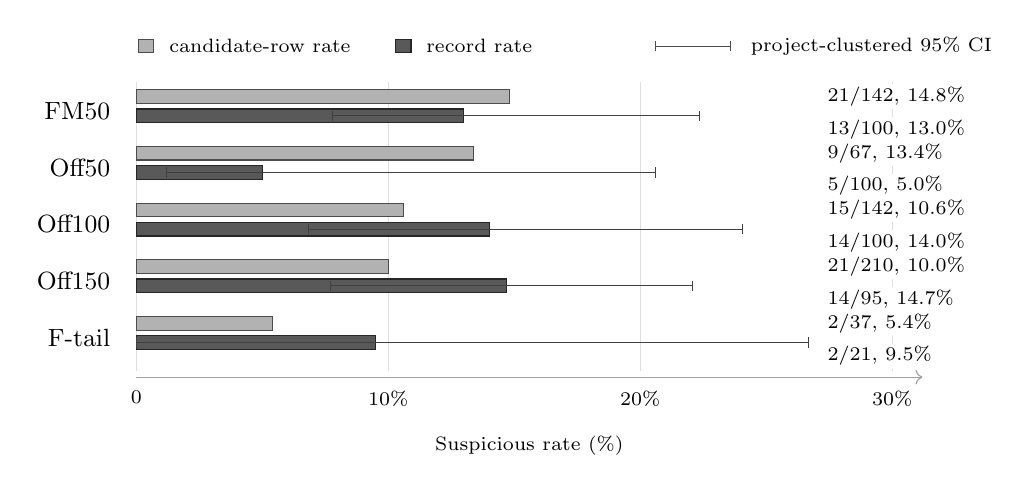
\begin{tikzpicture}[x=0.32cm,y=0.72cm,font=\small]
\draw[->,gray!75] (0,0.45) -- (31.2,0.45);
\node[font=\scriptsize] at (15.6,-0.75) {Suspicious rate (\%)};
\foreach \x/\lab in {0/0,10/10\%,20/20\%,30/30\%} {
  \draw[gray!25] (\x,0.55) -- (\x,5.65);
  \node[anchor=north,font=\scriptsize] at (\x,0.38) {\lab};
}

\filldraw[fill=black!30, draw=black!70] (0.1,6.18) rectangle (0.70,6.40);
\node[anchor=west,font=\scriptsize] at (0.92,6.29) {candidate-row rate};
\filldraw[fill=black!65, draw=black!85] (10.3,6.18) rectangle (10.90,6.40);
\node[anchor=west,font=\scriptsize] at (11.12,6.29) {record rate};
\draw[black!70,line width=0.35pt] (20.6,6.29) -- (23.6,6.29);
\draw[black!70,line width=0.35pt] (20.6,6.20) -- (20.6,6.38);
\draw[black!70,line width=0.35pt] (23.6,6.20) -- (23.6,6.38);
\node[anchor=west,font=\scriptsize] at (24.0,6.29) {project-clustered 95\% CI};

\node[anchor=east] at (-0.65,5.15) {FM50};
\filldraw[fill=black!30, draw=black!70] (0,5.28) rectangle (14.8,5.52);
\filldraw[fill=black!65, draw=black!85] (0,4.94) rectangle (13.0,5.18);
\draw[black!75,line width=0.35pt] (7.79,5.06) -- (22.35,5.06);
\draw[black!75,line width=0.35pt] (7.79,4.97) -- (7.79,5.15);
\draw[black!75,line width=0.35pt] (22.35,4.97) -- (22.35,5.15);
\node[anchor=west,font=\scriptsize,fill=white,inner sep=1pt] at (27.3,5.40) {21/142, 14.8\%};
\node[anchor=west,font=\scriptsize,fill=white,inner sep=1pt] at (27.3,4.82) {13/100, 13.0\%};

\node[anchor=east] at (-0.65,4.15) {Off50};
\filldraw[fill=black!30, draw=black!70] (0,4.28) rectangle (13.4,4.52);
\filldraw[fill=black!65, draw=black!85] (0,3.94) rectangle (5.0,4.18);
\draw[black!75,line width=0.35pt] (1.19,4.06) -- (20.59,4.06);
\draw[black!75,line width=0.35pt] (1.19,3.97) -- (1.19,4.15);
\draw[black!75,line width=0.35pt] (20.59,3.97) -- (20.59,4.15);
\node[anchor=west,font=\scriptsize,fill=white,inner sep=1pt] at (27.3,4.40) {9/67, 13.4\%};
\node[anchor=west,font=\scriptsize,fill=white,inner sep=1pt] at (27.3,3.82) {5/100, 5.0\%};

\node[anchor=east] at (-0.65,3.15) {Off100};
\filldraw[fill=black!30, draw=black!70] (0,3.28) rectangle (10.6,3.52);
\filldraw[fill=black!65, draw=black!85] (0,2.94) rectangle (14.0,3.18);
\draw[black!75,line width=0.35pt] (6.82,3.06) -- (24.05,3.06);
\draw[black!75,line width=0.35pt] (6.82,2.97) -- (6.82,3.15);
\draw[black!75,line width=0.35pt] (24.05,2.97) -- (24.05,3.15);
\node[anchor=west,font=\scriptsize,fill=white,inner sep=1pt] at (27.3,3.40) {15/142, 10.6\%};
\node[anchor=west,font=\scriptsize,fill=white,inner sep=1pt] at (27.3,2.82) {14/100, 14.0\%};

\node[anchor=east] at (-0.65,2.15) {Off150};
\filldraw[fill=black!30, draw=black!70] (0,2.28) rectangle (10.0,2.52);
\filldraw[fill=black!65, draw=black!85] (0,1.94) rectangle (14.7,2.18);
\draw[black!75,line width=0.35pt] (7.69,2.06) -- (22.09,2.06);
\draw[black!75,line width=0.35pt] (7.69,1.97) -- (7.69,2.15);
\draw[black!75,line width=0.35pt] (22.09,1.97) -- (22.09,2.15);
\node[anchor=west,font=\scriptsize,fill=white,inner sep=1pt] at (27.3,2.40) {21/210, 10.0\%};
\node[anchor=west,font=\scriptsize,fill=white,inner sep=1pt] at (27.3,1.82) {14/95, 14.7\%};

\node[anchor=east] at (-0.65,1.15) {F-tail};
\filldraw[fill=black!30, draw=black!70] (0,1.28) rectangle (5.4,1.52);
\filldraw[fill=black!65, draw=black!85] (0,0.94) rectangle (9.5,1.18);
\draw[black!75,line width=0.35pt] (0.0,1.06) -- (26.67,1.06);
\draw[black!75,line width=0.35pt] (0.0,0.97) -- (0.0,1.15);
\draw[black!75,line width=0.35pt] (26.67,0.97) -- (26.67,1.15);
\node[anchor=west,font=\scriptsize,fill=white,inner sep=1pt] at (27.3,1.40) {2/37, 5.4\%};
\node[anchor=west,font=\scriptsize,fill=white,inner sep=1pt] at (27.3,0.82) {2/21, 9.5\%};

\end{tikzpicture}
\caption{Detector-flagged suspicious dependency/import rates across the five Java APIHulBench windows. \codeid{FM50} combines 50 functional- and 50 method-split prompts; \codeid{Off50}/\codeid{Off100}/\codeid{Off150} are later offsets; \codeid{F-tail} is the final functional-split tail. Candidate-row rates are descriptive because rows are nested. Record-rate whiskers are project-clustered 95\% bootstrap intervals (10,000 replicates, seed 20260801)}
\label{fig:java-window-rates}
\end{figure}

Registry-feedback repair reduces suspicious imports but leaves residual detector-flagged cases in the first 3B Java window. The deterministic import-removal baseline removes all detector-flagged suspicious imports across all five 3B Java windows by applying the same rule used to define the removal target. We therefore report it as an auditable deletion baseline, not as independent proof that all dependency faults were verified and repaired. The original 7B Java control has no detector-flagged suspicious imports under enhanced mapping, so it contributes a zero-target, zero-edit sanitizer outcome rather than a repair-effect denominator. Under the 7B dependency-seeking B prompt, however, there are 6 targeted records with 8 flagged evidence rows. On these targets, C1 LLM feedback removes 4/4 invalid Maven/Gradle coordinate rows but leaves 4/4 suspicious import rows, reducing affected records from 6 to 2. C2 deterministic dependency sanitization removes both categories, reducing invalid coordinate rows from 4 to 0, suspicious import rows from 4 to 0, and affected records from 6 to 0. Under the stricter masked-import stress set, C1 feedback reduces the 4 detector-evidence records to 1 by lowering suspicious import rows from 4 to 1 and invalid coordinate rows from 1 to 0. C2 deterministic sanitization removes all 5 flagged evidence rows, reducing suspicious import rows, invalid coordinate rows, and affected records to 0.

Table~\ref{tab:mitigation-outcomes} reports repair/removal and all-window sanitizer outcomes.

\begin{table}[htbp]
\centering
\caption{Java repair and deterministic sanitizer outcomes. Panel A evaluates sequential LLM repair and detector-guided removal on the first 3B window. Panel B applies the deterministic sanitizer across all 3B windows; minimal-sentinel pass is descriptive and classpath-sensitive.}
\label{tab:mitigation-outcomes}
{\footnotesize
\setlength{\tabcolsep}{3pt}
\textit{Panel A: first-window repair and removal.}\par\smallskip
\begin{tabular}{@{}lccccc@{}}
\toprule
Method & Records & Candidates & Susp. rows & Susp. records & Susp. row reduction \\
\midrule
LLM repair round 1 & 13 & 40 $\rightarrow$ 9 & 21 $\rightarrow$ 4 & 13 $\rightarrow$ 4 & 0.810 \\
LLM repair round 2 & 4 & 7 $\rightarrow$ 3 & 4 $\rightarrow$ 2 & 4 $\rightarrow$ 2 & 0.500 \\
Deterministic sanitizer & 13 & 40 $\rightarrow$ 19 & 21 $\rightarrow$ 0 & 13 $\rightarrow$ 0 & 1.000 \\
\bottomrule
\end{tabular}
\medskip

\textit{Panel B: all-window deterministic sanitizer.}\par\smallskip
\begin{tabular}{@{}lccccc@{}}
\toprule
Window & Prompts & Candidates & Susp. rows & Susp. records & \shortstack{Minimal-sentinel\\post-removal pass} \\
\midrule
FM50 & 100 & 142 $\rightarrow$ 121 & 21 $\rightarrow$ 0 & 13 $\rightarrow$ 0 & 13 / 13 \\
FM50 offset 50 & 100 & 67 $\rightarrow$ 58 & 9 $\rightarrow$ 0 & 5 $\rightarrow$ 0 & 5 / 5 \\
FM50 offset 100 & 100 & 142 $\rightarrow$ 127 & 15 $\rightarrow$ 0 & 14 $\rightarrow$ 0 & 14 / 14 \\
FM50 offset 150 tail & 95 & 210 $\rightarrow$ 189 & 21 $\rightarrow$ 0 & 14 $\rightarrow$ 0 & 14 / 14 \\
F-only offset 200 tail & 21 & 37 $\rightarrow$ 35 & 2 $\rightarrow$ 0 & 2 $\rightarrow$ 0 & 2 / 2 \\
Combined & 416 & 598 $\rightarrow$ 530 & 68 $\rightarrow$ 0 & 48 $\rightarrow$ 0 & 48 / 48 \\
\bottomrule
\end{tabular}
}
\end{table}

Suspicious-row reduction is computed as \((\mathrm{pre} - \mathrm{post}) / \mathrm{pre}\) over detector-flagged suspicious import rows. The LLM repair rows are sequential: round 2 starts from the residual records left after round 1, which explains why it starts with 7 candidate rows rather than 40. For the 7B stress runs in Table~\ref{tab:java-protocols}, coordinate and import repairs are reported separately because LLM feedback and deterministic sanitization behave differently across the two evidence types. The 7B same-prompt control has no suspicious rows and therefore no sanitizer edits.

After sanitization across all five 3B windows, the combined Java candidate set contains 530 candidates and 0 suspicious import rows under the original detector taxonomy. The remaining mapped rows are 392 context/platform/project-local imports, 120 known external-prefix imports, 4 Maven class-search mappings, and 14 missing-import extractions. Against full human truth, the sanitizer deletes 66/101 invalid imports and retains 35/101 invalid imports; it incorrectly deletes 2/479 valid imports and correctly retains 477/479 valid imports. Thus it has high retention of valid rows but only 65.3\% coverage of invalid rows. For 7B, the same sanitizer is a no-op: the pre-sanitizer enhanced mapping already contains 374 no-external-needed rows and 4 known-prefix rows, with no suspicious rows to remove.

\subsubsection{Human-label error analysis}

We reuse the completed blind audit to quantify conservative handling errors. The audit covers all 598 extracted rows from the 3B Java sweep: 150 initial-audit rows and 448 annotation-held-out rows. Final labels contain 479 valid, 101 invalid, 15 malformed, and 3 uncertain rows. Annotator-specific sensitivity does not reverse the main result: A yields precision/recall/F1 0.971/0.653/0.781 on 580 evaluable rows; B yields 0.971/0.702/0.815 on 576; adjudicated truth yields 0.971/0.653/0.781 on 580. Table~\ref{tab:human-audit} also reports sanitizer deletion and retention against these labels.

Table~\ref{tab:human-audit} summarizes the human audit.

\begin{table}[htbp]
\centering
\caption{Completed Java human-audit results on the full 598 extracted-row 3B Java sweep.}
\label{tab:human-audit}
{\footnotesize
\setlength{\tabcolsep}{4pt}
\begin{tabularx}{\linewidth}{@{}lY@{}}
\toprule
Metric & Result \\
\midrule
Audit coverage & 598 / 598 rows annotated: 150 initial-audit rows and 448 annotation-held-out rows; 7 evaluation disagreements adjudicated \\
Inter-annotator agreement & Initial audit: 0 validity/subtype disagreements; evaluation validity 441 / 448 = 0.984, $\kappa=0.823$; evaluation subtype 440 / 448 = 0.982, $\kappa=0.973$ \\
Annotator sensitivity & A: P/R/F1 0.971/0.653/0.781 (580 evaluable); B: 0.971/0.702/0.815 (576); adjudicated: 0.971/0.653/0.781 (580) \\
Human validity counts & 101 invalid, 479 valid, 15 malformed, and 3 uncertain rows \\
Detector confusion matrix & TP 66, FP 2, FN 35, TN 477 on 580 valid/invalid rows \\
Post-extraction classification precision & 66 / 68 = 0.971; project-clustered 95\% CI 0.921--1.000 \\
Post-extraction classification recall & 66 / 101 = 0.653; project-clustered 95\% CI 0.526--0.792 \\
Post-extraction classification F1 & 0.781; project-clustered 95\% CI 0.680--0.874 \\
Raw-response audit coverage & 416 / 416 responses; 1,026 adjudicated mentions; exact mention-sequence agreement on 370 / 416 responses; 146 records adjudicated \\
Frozen extractor & TP/FP/FN 589/9/437; precision 0.985 (95\% CI 0.962--0.998), recall 0.574 (0.530--0.626), F1 0.725 (0.688--0.766) \\
Hybrid grounded end-to-end detector & Invalid/malformed TP/FP/FN 66/2/249; precision 0.971 (95\% CI 0.920--1.000), recall 0.210 (0.151--0.291) \\
Raw-response-only sensitivity & TP/FP/uncertain/FN 15/6/47/257; known-label precision 0.714, recall 0.055 \\
Sanitizer on human-invalid rows & 66 / 101 deleted; 35 / 101 retained (invalid-import coverage 0.653) \\
Sanitizer on human-valid rows & 2 / 479 incorrectly deleted; 477 / 479 correctly retained (valid-import retention 0.996) \\
Malformed/uncertain handling & 15 malformed rows and 3 uncertain rows are excluded from precision/recall/F1 denominators \\
\bottomrule
\end{tabularx}
}
\end{table}

Table~\ref{tab:mapping-human-cross} cross-tabulates detector status and final human labels.

\begin{table}[htbp]
\caption{Detector mapping status crossed with final human validity labels for all 598 Java candidate rows.}
\label{tab:mapping-human-cross}
{\footnotesize
\setlength{\tabcolsep}{3pt}
\begin{tabularx}{\linewidth}{@{}Yrrrrr@{}}
\toprule
Detector mapping status & Valid & Invalid & Malformed & Uncertain & Total \\
\midrule
\codeid{no_external_mapping_needed} & 365 & 23 & 1 & 3 & 392 \\
\codeid{mapped_known_prefix} & 109 & 11 & 0 & 0 & 120 \\
\codeid{mapped_maven_class_search} & 3 & 1 & 0 & 0 & 4 \\
\codeid{project_namespace_hallucination} & 0 & 34 & 0 & 0 & 34 \\
\codeid{project_namespace_typo_hallucination} & 0 & 13 & 0 & 0 & 13 \\
\codeid{hallucinated_prefix_with_suggestion} & 0 & 14 & 0 & 0 & 14 \\
\codeid{unresolved_after_mapping} & 2 & 5 & 0 & 0 & 7 \\
\codeid{missing_import} & 0 & 0 & 14 & 0 & 14 \\
\midrule
Total & 479 & 101 & 15 & 3 & 598 \\
\bottomrule
\end{tabularx}
}
\end{table}

Table~\ref{tab:mapping-human-cross} resolves the apparent 14-versus-15 malformed discrepancy. All 14 \pathid{missing_import} rows are human-labeled malformed. The additional malformed row is full-sweep index 233, \pathid{com.tencent.supersonic.headless.api.pojo.request.QueryReq.Req.}. Its trailing dot makes the import syntactically incomplete; the original mapper placed it under \pathid{no_external_mapping_needed} because its broader classification was project-local.

The same cross-table localizes the 35 false negatives: 23 are under \pathid{no_external_mapping_needed}, 11 under \pathid{mapped_known_prefix}, and 1 under \pathid{mapped_maven_class_search}. The two sanitizer false deletions, \pathid{reactor.core.publisher.Mono} and \pathid{com.alibaba.fastjson.JSON}, are both in \pathid{unresolved_after_mapping}.

We evaluate the three frozen recall-extension checks separately on the 150 rule-development rows and the remaining 448 annotation-held-out rows. Wildcard platform imports remain excluded because \codeid{javap} resolves classes rather than packages. Table~\ref{tab:recall-extension} reports the development, evaluation, and descriptive overall partitions.

\begin{table}[htbp]
\centering
\caption{Frozen recall-extension evaluation. Dev is the 150-row rule-development partition; Eval is the 448-row annotation-held-out partition. TP, FP, FN, and TN denote true positives, false positives, false negatives, and true negatives against final human labels. Eval is row-level, not project-disjoint; the 598-row result is descriptive. Metrics exclude malformed and uncertain rows.}
\label{tab:recall-extension}
{\footnotesize
\setlength{\tabcolsep}{2.5pt}
\begin{tabular}{@{}lrrrrrrrr@{}}
\toprule
Partition & Eligible & TP & FP & FN & TN & Precision & Recall & F1 \\
\midrule
Development 150 & 135 & 82 & 2 & 0 & 51 & 0.976 & 1.000 & 0.988 \\
Annotation-held-out 448 & 445 & 16 & 28 & 3 & 398 & 0.364 & 0.842 & 0.508 \\
Overall 598 (descriptive) & 580 & 98 & 30 & 3 & 449 & 0.766 & 0.970 & 0.856 \\
\bottomrule
\end{tabular}
}
\vspace{0.35em}

{\footnotesize
\begin{tabularx}{\linewidth}{@{}Yrrrrrrr@{}}
\toprule
Added rule & Dev add & Dev TP & Dev FP & Eval add & Eval TP & Eval FP & Eval precision \\
\midrule
Known external class & 9 & 9 & 0 & 27 & 3 & 24 & 0.111 \\
Platform class & 5 & 5 & 0 & 13 & 9 & 4 & 0.692 \\
Project/context class & 2 & 2 & 0 & 4 & 4 & 0 & 1.000 \\
\bottomrule
\end{tabularx}
}
\end{table}
 
The annotation-held-out row-level result does not support the recall extension as a general detector improvement. It recovers 16/19 evaluation-partition false negatives but adds 28 false positives, yielding precision 0.364 and F1 0.508. The failure is concentrated in the external-class rule: its development precision is 9/9, but its evaluation precision is only 3/27. The project-source rule remains correct on 4/4 evaluation additions, and the platform rule is correct on 9/13. The 598-row figures (precision 0.766, recall 0.970, F1 0.856) are therefore retained only as descriptive accounting, not final validation. Project overlap further precludes an external-generalization interpretation. This ablation identifies a useful project-source check and a partially useful platform check, but it rejects local-jar absence under a known external prefix as a stand-alone invalidity rule. The import-only probe over the 60 added rows still fails before removal and passes afterward in 38/38 records; because 28 added rows are human-labeled valid, that result demonstrates classpath sensitivity rather than detector correctness.

Table~\ref{tab:import-only-control} reports the import-only sentinel control.
\begin{table}[htbp]
\caption{Same-protocol import-only control probe on detector-flagged and unflagged Java audit samples. Candidate-import pass reports whether the sentinel containing the sampled imports compiled; empty baseline reports the same sentinel shell after removing all sampled imports.}
\label{tab:import-only-control}
{\footnotesize
\begin{tabularx}{\linewidth}{@{}lrrYY@{}}
\toprule
Group & Rows & Records & Candidate-import outcome & Interpretation \\
\midrule
Detector-flagged imports & 68 & 48 & Candidate imports pass in \rate{0}{48}; empty baseline passes in \rate{48}{48}. & All detector-flagged records fail under the minimal probe. \\
Unflagged controls & 68 & 53 & Candidate imports pass in \rate{16}{53} (30.2\%); empty baseline passes in \rate{53}{53}. & The remaining 37/53 fail, mostly from absent classpaths or unflagged invalid imports. \\
\bottomrule
\end{tabularx}
}
\end{table}

These probes provide bounded import-resolution and injected-import compilation-impact evidence. In the Maven probe, 12/14 interpretable target pairs from 8/10 build units fail after suspicious-import injection and pass after sanitizer removal, and all 14 sanitized variants pass \codeid{test-compile}. The two injected-pass pairs show that project-level impact depends on build configuration. The import-only compiler probe covers all 48 original suspicious-import records across the combined 3B Java run: raw suspicious-import sentinels fail under \codeid{javac} in 48/48 records, while sanitized sentinels compile in 48/48. The recall-extension import-only probe shows the same fail-then-pass pattern on the 38 records containing newly added candidates. However, Table~\ref{tab:import-only-control} shows that the same minimal protocol also fails for 37/53 unflagged-control records. Failure categories in the control run include package-missing or classpath-absent diagnostics for 33 records, cannot-find-symbol diagnostics for 2 records, malformed-import syntax for 1 record, and 1 other \codeid{javac} failure. We therefore interpret import-only results as classpath-sensitive evidence rather than detector accuracy, and the Maven result only as an injected-import compilation probe. Neither probe establishes full generated-code correctness, unresolved-symbol reduction in model completions, or test-suite success.

\section{Discussion}

The results suggest that dependency hallucination should be treated as an engineering measurement problem rather than a single model-output property. The same generated text may contain installable packages, standard-library references, module paths, project-local symbols, valid external imports, and fabricated dependency names. A detector that collapses all of these cases into one hallucinated label risks obscuring the cause of failures. Conversely, a detector that only checks package registry membership can miss import-level failures that matter in compiled languages.

The Python results illustrate the value of layered measurement. Raw rates preserve comparability with the original Package Hallucination protocol. Artifact-filtered rates remove malformed outputs. Deterministic post-labeling then stratifies detected mentions into registry-missing candidates, module paths, standard-library tokens, ecosystem aliases, or parser artifacts. This is useful error decomposition, but unlike the Java analysis it is not independent two-annotator truth.

The Java results show why dependency hallucination cannot be reduced to package recommendation alone. Generated Java code often expresses dependency assumptions through import statements. Some imports are harmless because they refer to platform classes, prompt-provided context, or project-local source files. Others are suspicious because they mimic the project namespace without a matching class, contain a namespace typo, or use an external-library prefix that does not correspond to the expected dependency. These cases are not captured by Maven-coordinate validation alone. They require project-source grounding and an import-aware taxonomy.

The original Java 7B full-sweep control is not mitigation evidence. On the same 416 original-protocol prompts, Qwen-7B produces fewer dependency candidates and no detector-flagged suspicious imports under enhanced mapping. The 3B suspicious-import rate should therefore not be generalized to 7B. The dependency-seeking prompt exposes 6 records with confirmed invalid dependency evidence, while the original masked protocol recovers 34/160 targets as parseable import rows. In the test-compile-gated subset, generated import evidence restores 14/83 masked gold-code sources. The post-pilot structured diagnostic reports the full and non-repeated-context matrices separately; all three observed end-to-end test-compilation passes are in the non-repeated cohort. This removes repeated-context leakage as an explanation for those three cases, but pilot/final overlap still prevents an independent performance claim. The non-unified DeepSeek run remains confined to Appendix~\ref{app:format-sensitivity} and is not used for model ranking.

The human audit shows that validity classification is precise but incomplete among the extracted Java rows. The 66/68 invalid classifier-flagged rows support the registry/project taxonomy as a high-precision signal, while the 35 invalid unflagged extracted rows expose a post-extraction classification-recall limitation. The completed raw-response audit adds the missing upstream accounting: the extractor has high precision (0.985) but only 0.574 recall, and the frozen end-to-end detector recalls 0.210 of human-invalid or malformed mentions. Most extractor misses occur in malformed expressions (173/437) and broken fences (156/437), with additional ordinary-code, prose, and other-surface misses. The result is a useful boundary finding: downstream classification is precise conditional on extraction, but extraction coverage is the dominant end-to-end limitation. The annotation-held-out row-level ablation prevents an overly favorable interpretation of the recall extension: although it recovers 16/19 evaluation-partition false negatives, it also adds 28 false positives, and the known-external class rule has evaluation precision 3/27. Only the project-source rule remains perfect on its small evaluation set (4/4), while the platform rule reaches 9/13. Because 47 projects overlap between development and evaluation rows, this is not project-disjoint validation. The result is therefore a boundary finding, not an improved final detector. The unflagged-control compiler probe reinforces the same caution: minimal \codeid{javac} failures are sensitive to incomplete classpaths and cannot substitute for human truth or project builds.

The repair/removal experiments are diagnostic baselines, not evidence that either intervention improves software quality. In the first 3B Java window, registry-feedback repair reduces detector-flagged mentions in the observed outputs. In the 7B dependency-seeking run, it removes all 4 confirmed invalid coordinates but repeats all 4 suspicious imports; in the masked-import run, it reduces evidence records from 4 to 1. These small, selected denominators do not establish reliable repair performance. The deterministic sanitizer removes detector-flagged rows by construction, but the human audit shows that this rule misses 35/101 invalid rows and deletes 2/479 valid rows. Its apparent reduction in flagged counts is therefore not an independent effectiveness result, and neither intervention has been shown to improve functional correctness, test outcomes, or developer workflows.

The prospective results change the practical interpretation. V2 closes part of the extraction gap and raises external end-to-end recall from 0.103 to 0.504, but its 0.319 precision means most flags are not confirmed invalid/malformed mentions. A tool should therefore retain raw text and span provenance, expose the evidence and rule for each candidate, and present V2 as a review queue. Automatic deletion is not justified. V1 remains a conservative comparator, but its external recall of 0.103 makes it unsuitable as a comprehensive screen. The two versions expose a precision--recall trade-off rather than a deployable winner.

The human results also caution against treating a single annotation sheet as complete. Although matched-label kappa is high, mention-enumeration F1 is only 0.499 and 262/543 final occurrences remain uncertain under conservative adjudication. Broken text, simple identifiers, and repeated mentions are genuine measurement difficulties. Reporting both enumeration agreement and matched-label agreement prevents good label consistency from masking poor agreement about which mentions exist.

The legacy third-party return changes the point estimates but does not reverse the deployment conclusion: V2 remains below both the precision and recall gates. Since that workbook contains no separate dependency-mention decision and its filled values exactly match a row-indexed scripted template, we retain its scores only as a sensitivity analysis and do not claim independent third-expert validation or a passed hidden-control QC gate. The original frozen evaluation remains the primary analysis.

The engineering stop is informative for practice. Only two of 30 independently selected projects pass a nonzero baseline suite in the available environment, despite fixed commits and root Maven POMs. This prevents the planned four-variant intervention from reaching its minimum denominator and shows that buildability is a selection and transportability problem of its own. Prior large-scale Java studies likewise find that automatic buildability and the availability of nonzero tests are substantial sampling constraints rather than routine prerequisites.\citep{Hassan2017AutomaticBuild,Khatami2024QA} Future practice-effect work needs a separately frozen, build-eligible sampling frame or a containerized upstream environment, while still counting every screened failure. The present evidence supports human-in-the-loop auditing and measurement, not autonomous mitigation or demonstrated developer-workflow benefit.

The rule-level error analysis is diagnostic, not a license to tune V2 on the 200-answer external set. Any V3 that disables the broad malformed-import path or retains only higher-precision namespace-typo evidence would be developed with knowledge of these labels. It must therefore be frozen and tested on a new project-, owner-, and API-family-disjoint holdout before being compared with the preregistered V1/V2 results.

\section{Threats to Validity}

\textbf{Construct validity.} Dependency hallucination is a broad concept. A missing package name, a non-existent import path, a wrong project namespace, and an unavailable API are related but not identical. We address this threat with a fine-grained taxonomy and a completed audit of all 598 Java rows. The masked-import textual metric is intentionally strict: a hidden import is recovered only when its full name appears in a parseable dependency row. V2 validates generated import sets against original code under \codeid{test-compile}; the exploratory 2-by-2 diagnostic separately inserts generated spans and generated imports. All 12 overall compilation-valid model-code spans are reference-exact, but reference equality and test-compilation do not imply semantic correctness or a complete Maven lifecycle. The full-sweep audit retains 15 malformed and 3 uncertain rows outside precision/recall/F1 denominators. Two non-author annotators complete independent external sheets, but mention-enumeration F1 is only 0.499; high matched-label kappa does not remove inventory uncertainty. The conservative adjudication leaves 262 mentions uncertain and reports both extreme-label sensitivities. A supplementary legacy third-party return relabels these target occurrences but lacks the protocol's separate dependency-mention decision and cannot be treated as a QC-certified adjudication; its metrics are reported only as a sensitivity analysis. Local-jar absence alone is insufficient for an invalid label.

\textbf{Extraction validity.} The candidate-row audit begins after the Java extractor has converted the 416 raw model responses into 598 rows, so its 0.653 recall remains a post-extraction classification metric. The completed raw-response audit independently reviews all 416 responses using two detector-blind blank sheets and adjudicates 146 rows with any core-field difference. It finds extractor precision/recall/F1 of 0.985/0.574/0.725. The primary end-to-end precision/recall of 0.971/0.210 uses a hybrid grounded truth: extracted mentions use the separately completed project/registry-grounded candidate labels for validity, while unextracted mentions use raw-response adjudication. Under raw-response validity labels alone, TP/FP/uncertain/FN are 15/6/47/257, with known-label precision 0.714 and recall 0.055. The estimates remain descriptive over the observed 97 project paths and do not establish external generalization. Credential-redacted raw generation records, blank templates, completed annotator sheets, adjudication audit, scoring script, and clustered bootstrap draws are preserved so that both the local and prospective results can be audited without rerunning the models. In the prospective set, V2 extraction precision/recall are 0.523/0.374, so extraction remains a limiting layer even after the frozen format extension.

\textbf{Internal validity.} Python post-labeling uses deterministic rules over package names, standard-library names, module paths, and ecosystem aliases; it has no Java-style independent human audit. Ambiguous identifiers may be misclassified, so we preserve raw detector output and report rule-stratified outcomes separately. The original Java classifier rules were refined while all five candidate windows were observable, and no independent test split or separately recorded original-classifier freeze timestamp exists. Script and candidate-export hashes identify the snapshot, and its 0.971/0.653/0.781 metrics are an in-corpus post-extraction classifier characterization. The grounding ablation is a diagnostic coverage-first contrast, not a comparison of independently trained detectors. For the recall-extension ablation, labels rather than projects are held out: the 150-row development and 448-row evaluation partitions share 47 projects. For structured V3, a 35-record pilot exposed an incorrectly scoped import instruction. The corrected rerun uses separate paths and hashes, but development and final records overlap; its matrices are explicitly post-pilot exploratory and may include prompt-refinement optimism. In contrast, prospective V1/V2 code, prompts, parameters, selection rules, and scoring code are hash-frozen before acquisition; no external label changes either pipeline. One operational deviation affects only the engineering harness: after freezing and before complete baseline screening, its Windows timeout handler was changed to terminate the Maven process tree and return promptly. Selection, Maven goals, timeout threshold, eligibility, parsing, and outcome classification were unchanged; frozen and executed hashes are preserved. No intervention or practice-effect estimate follows from this harness. The conservative adjudication protocol is detector-blind but is specified after annotator disagreement is observed, so its sensitivity analyses are essential.

\textbf{External validity.} The prospective evaluation supplies a project-disjoint estimate over 30 fixed-commit Java/Maven repositories and 200 answers, but it is still one model, one deterministic decoding configuration, two prompt arms, and one GitHub search snapshot. Name, full-name, and owned API-family exclusions cover all 97 local projects; owner provenance is mapped for only 79/97, so owner disjointness cannot be proven for 18 local projects. Invalid/malformed mentions occur in 12/30 external projects, producing wide project-clustered intervals. Eleven immediate-EOS responses are retained, which preserves intention-to-treat validity but may lower observed candidate production. These results do not generalize to other languages, models, sampling frames, or interactive developer use. The earlier 8-repository/16-record study remains only an appendix protocol trial because it used name-level deduplication and source/build/API labels rather than independent blank sheets.

\textbf{Registry validity.} Registry snapshots and local dependency caches change over time. A package that is missing in one PyPI or Maven snapshot may later be registered, and package names may also be removed or renamed. The recall extension relies on a local Maven jar class index; an incomplete local cache can miss valid external classes, while a broader cache can resolve more classes. For the DeepSeek masked-import format-sensitivity control, external Maven querying was not run after privacy review because generated coordinates include project-derived identifiers. We therefore label only local Maven-cache hits and obvious placeholder/missing coordinates in that run, and we do not infer registry absence from local-cache absence. We preserve validation outputs and report the local jar-index size so that results can be interpreted relative to the exact registry and cache evidence used in the experiment.

\textbf{Compilation and test validity.} The injected-import probe yields 14 interpretable pairs from 10 baseline-passing units: 12 pairs from 8 units fail after injection and pass after removal. The masked-import validation starts from 85 units; 58 units covering 83 records pass V0, while 27 are excluded for documented baseline failures. V2 inserts imports into gold code and passes \codeid{test-compile} in 14/83 records. The exploratory 2-by-2 diagnostic yields 3/83 end-to-end test-compilation passes overall and 3/75 after removing repeated-context prompts. Maven \codeid{package}/\codeid{verify} is not run. Only 10/58 baseline units pass while executing nonzero tests. Their intersection with the 14 V2 compilation-valid records is 0, and none covers a structured end-to-end pass. Therefore neither result has an eligible project-test denominator, and no test-pass proportion is estimable. The import-only probe remains classpath-sensitive and is not detector-accuracy evidence. In the prospective engineering screen, only 2/30 projects pass a nonzero baseline suite and the remaining frozen snapshot yields no additional eligible repository. Because the preregistered eight-project minimum fails before mutation, no four-variant practice-effect outcome exists; this is a feasibility result, not evidence that deletion or repair is ineffective.

The real-test sanitizer probe supplies baseline-restoration evidence only for the removal operation. Five injected imports fail before tests; after exact removal, all five copies return to the original source and match the baseline outcome across five paired records, three projects, and 451 unique baseline tests. This does not establish correctness of generated replacement code, semantic equivalence for arbitrary projects, or safety when a detector misses a required import.

\textbf{Repair/removal validity.} The deterministic sanitizer removes detector-flagged suspicious dependency mentions and invalid coordinates, but it does not synthesize missing correct code, infer all required dependencies, or prove semantic correctness. In the masked-import stress set, sanitization removes flagged evidence without improving the exact hidden-import recovery rate, which remains 34/160. Its purpose is therefore narrower: provide a reproducible dependency-cleaning baseline. LLM repair may be more flexible, but the current residual cases show that self-repair can be unstable even with explicit feedback.

\section{Reproducibility Package}

The confidential review artifact preserves credential-redacted raw generation records, extracted candidates, the completed local and prospective raw-response mention-audit packages, validation labels, mitigation outputs, completed human-audit files, annotator agreement and sensitivity metrics, prospective V1/V2 scores and claim gates, engineering eligibility and stop records, full-598 local truth labels, recall-extension outputs, grounding-source ablation outputs, masked-import nesting statistics, original and structured build matrices, real-test baselines, project-clustered bootstrap draws, Java build-provenance hashes, reported compiler/build logs, frozen runner scripts, model identifiers, prompt-selection offsets, registry snapshots, and environment notes. A standard-library one-command core recomputation regenerates seven submission-critical analyses and asserts 40 selected paper values, including the grounding-source ablation and raw-response audit; other reported values are indexed to preserved source artifacts in the final manifest. The final archive is accepted only after this command passes in a newly extracted directory and an anonymity scan finds no local account names or submission-author identifiers, drive-letter paths, absolute paths, cache dependencies, or copied project trees. The invalid structured pilot is clearly separated from the corrected reported run. This separation of review-only evidence, public-safe aggregates, provenance, and explicit access constraints follows published recommendations for open empirical-software-engineering artifacts.\citep{Runeson2024OpenArtifacts}

Artifact-relative paths and corresponding file hashes are maintained in the manifest. This keeps the manuscript focused on the experimental claims while preserving portable, anonymous traceability for reproduction.

\textbf{Responsible artifact release.} The review artifact is intended for confidential editorial and peer-review use because some raw outputs include registry-missing dependency names that could be misused as package-confusion candidates. A public artifact release should hash or redact registry-missing package names unless they are already safely registered or otherwise cleared, and should preserve the full names only in a controlled-access review archive.

\section{Conclusion}

This paper presents an auditable dependency-hallucination measurement workflow and separates extraction, conditional classification, and end-to-end detection. The original 97-project corpus shows high post-extraction classification precision (0.971) but low end-to-end recall (0.210). In the frozen prospective evaluation, two independent annotators review 200 answers from 30 new repositories. V2 improves end-to-end recall from V1's 0.103 to 0.504, with a positive project-clustered recall-difference interval, but precision falls from 0.857 to 0.319. The large uncertainty stratum and wide project intervals reinforce the same conclusion: V2 is a recall-oriented review aid, not an autonomous detector prototype.

The engineering upgrade also fails its preregistered eligibility gate. Only two external projects pass nonzero baseline tests, and screening all 386 remaining ranked entries in the frozen snapshot yields no additional eligible repository. Consequently, no four-variant intervention or practice-effect claim is reported. Together with the bounded local compilation and sanitizer probes, the evidence supports registry-, project-, and human-grounded auditing and measurement. It does not establish safe automatic deletion, functional correctness, developer benefit, or broad ecosystem generalization.

The supplementary legacy-label sensitivity analysis also leaves V2 below both the preregistered precision and recall gates. Because the legacy return lacks a separate dependency-mention decision and cannot be treated as an independently quality-controlled adjudication, the frozen two-annotator inventory remains the primary external result.

\section*{Statements and Declarations}

\subsection*{Funding}

No external funding was received for this work.

\subsection*{Competing Interests}

The authors declare no competing interests.

\subsection*{Author Contributions}

Haonan Wang: experimental implementation, data collection and analysis, initial manuscript drafting, and figure and table preparation. Shiyong Xiong: study conception, research-plan design, manuscript revision and approval, submission coordination, and overall responsibility for the paper. Both authors approved the submitted version and accept accountability for the work.

\subsection*{Ethics Approval}

This study did not require ethics approval because no personal or sensitive information was collected. The two annotators provided informed consent for the annotation activity.

\subsection*{Informed Consent}

The two annotators provided informed consent and received no compensation. No personal or sensitive information was collected. Their row-level annotations are not authorized for public release.

\subsection*{Data Availability}

The two annotators provided informed consent and received no compensation; they did not authorize public release of their row-level annotations.

The manuscript source and study-authored public materials will be available at https://github.com/whaonan767-tech/paper. The public sanitized artifact will be archived at a persistent DOI (DOI: AUTHOR INPUT REQUIRED). The public release excludes raw prompts and responses, row-level annotations and adjudication, registry-missing candidate lists, compiler logs, third-party project trees, local model weights, and package-manager caches. The complete review artifact contains additional row-level evidence and is supplied only through the journal's confidential editorial system, subject to contributor and third-party data restrictions. Exact compilation reruns require lawful acquisition of the APIHulBench authors' official project archive and verification of all 70 content-addressed project revisions; this paper does not redistribute those trees, including the 19 snapshots with no discoverable license document. The public artifact supports the aggregate checks described in its README but does not independently reproduce analyses requiring excluded row-level data.

The review artifact additionally includes the prospective 30-repository acquisition snapshot and fixed-commit manifest, all 200 redacted Qwen-3B responses, both completed blank-sheet exports, agreement and conservative adjudication records, frozen V1/V2 candidates and decisions, 10,000 project-clustered bootstrap draws, claim-gate assertions, all 30 baseline build logs, the 386-rank extension screen, and the engineering stop record. The earlier 8-repository/16-record protocol trial is retained separately in the appendix package.

\section*{Author Biographies}

Haonan Wang is a graduate student in the School of Computer Science at Chongqing University of Posts and Telecommunications. Wang's research interests include software architecture and software quality, particularly the reliability and measurement of dependencies in AI-generated code.

Shiyong Xiong is a professor-level senior engineer and master's supervisor at Chongqing University of Posts and Telecommunications. He is Director of the Institute of Digital Media Technology and leader of the Digital Media Research and Innovation Team in the School of Computer Science. His research interests include software engineering, digital media processing, image visualization, and software system architecture. He is a nationally certified systems architect and holds an Oracle certification. He combines academic research with engineering practice and serves as a technical consultant to the Chongqing municipal government and several large enterprises. He has led or participated in more than ten national or provincial/ministerial research projects and has led his team in completing more than fifty commissioned engineering projects. He has published research papers and books in related areas, with a focus on image processing, digital media, and software architecture.

\appendix

\section{Eight-Repository Protocol Trial}
\label{app:external-pilot}

Before the prospective study, a frozen 16-answer trial over eight previously unused repositories exercised acquisition, Qwen-3B generation, extraction, mapping, and scoring. Source/build/API grounding gave TP/FP/FN/TN = 3/1/0/12, and a cold/warm mapping benchmark took 66.596/0.292 seconds. The trial selected by repository name only, included two repositories from an API family present in the local corpus, lacked independent blank-sheet annotation, and encountered unavailable builds. It is retained solely as a protocol and artifact-pipeline test; it is not used in the abstract, main external metrics, or generalization claims.

\section{Post-Pilot Structured Diagnostic}
\label{app:structured-diagnostic}

Table~\ref{tab:masked-v3-factorial} separates generated-code and generated-import contributions under the same structured output. The non-repeated cohort excludes exactly eight prompts with another visible occurrence of the reference span. Because protocol development and final records overlap, the matrix is supplementary diagnostic evidence rather than a held-out performance estimate.

\begin{table}[htbp]
\centering
\caption{Post-pilot exploratory same-output 2-by-2 test-compilation results. Tests are compiled but not executed.}
\label{tab:masked-v3-factorial}
{\footnotesize
\setlength{\tabcolsep}{4pt}
\begin{tabularx}{\linewidth}{@{}lllrrY@{}}
\toprule
Context & Code & Imports & Pass & Fail & Project-clustered 95\% CI \\
\midrule
All 83 & Gold & Gold & 83 & 0 & Eligibility baseline \\
All 83 & Gold & Model & 13 & 70 & 6.7--25.0\% \\
All 83 & Model & Gold & 12 & 71 & 5.4--23.9\% \\
All 83 & Model & Model & 3 & 80 & 0.0--8.3\% \\
Non-repeated 75 & Gold & Gold & 75 & 0 & Eligibility baseline \\
Non-repeated 75 & Gold & Model & 12 & 63 & 6.3--26.0\% \\
Non-repeated 75 & Model & Gold & 9 & 66 & 4.2--20.7\% \\
Non-repeated 75 & Model & Model & 3 & 72 & 0.0--9.6\% \\
\bottomrule
\end{tabularx}
}
\end{table}

\section{Compiler-Probe Accounting}
\label{app:compiler-probes}

Table~\ref{tab:compiler-probes} reports the detailed coverage and outcomes of the injected-import Maven probe and minimal \codeid{javac} sentinels. These are compilation-facing diagnostics; the Maven goal skips test execution and the import-only probe uses incomplete classpaths.

\begin{table}[htbp]
\centering
\caption{Detailed compiler-facing probe summary.}
\label{tab:compiler-probes}
{\footnotesize
\begin{tabularx}{\linewidth}{@{}L{48mm}Y@{}}
\toprule
Metric & Result \\
\midrule
Maven probe coverage & 38 window-specific baseline runs; 36 unique build units from 34 projects across five Java windows \\
Maven baseline outcomes & 11 pass runs / 10 units; 27 failed runs / 26 units: toolchain 19 / 18, dependency resolution 6 / 6, other 2 / 2 \\
Maven interpretable targets & 14 target pairs from 10 independent baseline-passing build units \\
Maven injected fail/removal pass & 12 / 14 pairs from 8 / 10 build units; descriptive paired outcome \\
Maven injected pass/removal pass & 2 / 14 pairs from 2 / 10 build units \\
Maven sanitized variants & 14 / 14 interpretable target pairs pass \codeid{test-compile} \\
Import-only original targets & 68 rows in 48 detector-flagged records; raw sentinels fail in 48 / 48 and sanitized sentinels pass in 48 / 48 \\
Recall-extension candidates & 60 rows in 38 records; raw added-candidate sentinels fail in 38 / 38 and sanitized sentinels pass in 38 / 38 \\
\bottomrule
\end{tabularx}
}
\end{table}

\section{Non-Unified Model Format Sensitivity}
\label{app:format-sensitivity}

This appendix preserves the DeepSeek-Coder-6.7B-Instruct run without treating it as a model-quality comparison. Both models receive the same 117 masked-import prompts, but Qwen-7B uses a 512-token cap, the default chat/system configuration, and the main validation pipeline, whereas DeepSeek uses a 1024-token cap, no system message, a tokenizer-file backend, and offline-only coordinate validation. Strict observed manifest-format compliance requires a closed \codeid{java} fence, a \codeid{Dependencies:} heading, and at least one recognized dependency row or no-dependency response.

Table~\ref{tab:appendix-format} reports appendix-only format diagnostics.

\begin{table}[htbp]
\centering
\caption{Format and output-length diagnostics for the non-unified masked-import runs. Cap is the token cap; mean/med. is mean/median decoded tokens after re-encoding; Ceiling proxy counts responses within two tokens of the cap and is not a recorded finish reason.}
\label{tab:appendix-format}
{\footnotesize
\setlength{\tabcolsep}{3pt}
\begin{tabular}{@{}lrrrrr@{}}
\toprule
Model & Cap & Strict format & Import records & Tokens mean/med. & Ceiling proxy \\
\midrule
Qwen-7B & 512 & 101/117 (86.3\%) & 39/117 (33.3\%) & 109.5/85 & 1/117 (0.9\%) \\
DeepSeek-6.7B & 1024 & 12/117 (10.3\%) & 2/117 (1.7\%) & 295.6/249 & 7/117 (6.0\%) \\
\bottomrule
\end{tabular}
}
\end{table}

The historical runner did not preserve generation token IDs or finish reasons. The ceiling proxy therefore counts a decoded response only when re-encoding places it within two tokens of the configured cap; it is not a recorded truncation reason. DeepSeek shows lower observed manifest-format compliance under these conditions, but the unequal cap, system-message setting, tokenizer path, and validation scope prevent attributing its 1/160 strict recovery result to weaker dependency knowledge. The value is not used in the abstract, contributions, or main conclusion. The updated runner records generated token count, EOS emission, and finish reason for future controlled runs.

\section{Injected-Import Build Units}
\label{app:build-units}

Table~\ref{tab:appendix-build-units} lists the baseline-passing Maven build units.

\begin{table}[htbp]
\centering
\caption{All 10 unique baseline-passing build units in the preserved injected-import Maven probe. The \codeid{jar-analyzer} unit appears in two window-specific baseline runs, producing 11 pass rows in total.}
\label{tab:appendix-build-units}
{\footnotesize
\setlength{\tabcolsep}{3pt}
\begin{tabularx}{\linewidth}{@{}lYrl@{}}
\toprule
Project & Build unit & Targets & Injected/removal outcome \\
\midrule
\codeid{akto-vv1.30.0} & \codeid{libs/dao} & 1 & fail/pass \\
\codeid{campus-v1.1.10} & \codeid{campus-common} & 1 & fail/pass \\
\codeid{crane4j-v2.7.0} & \codeid{crane4j-core} & 1 & fail/pass \\
\codeid{easy-rpc-main} & \codeid{easy-rpc-core} & 2 & 2 fail/pass \\
\codeid{easy-task-scheduler-main} & \codeid{scheduler-admin} & 1 & pass/pass \\
\codeid{flowlong-dev} & \codeid{flowlong-core} & 1 & fail/pass \\
\codeid{jar-analyzer-2.15} & project root & 4 & 4 fail/pass \\
\codeid{JNDIMap-main} & project root & 1 & fail/pass \\
\codeid{mePush-main} & \codeid{xxl-job-admin} & 1 & pass/pass \\
\codeid{TaSK-1.0.1} & \codeid{task.xmlparser} & 1 & fail/pass \\
\bottomrule
\end{tabularx}
}
\end{table}

Across all 38 window-specific baseline runs (36 unique build units), the 27 failures represent 26 unique units and comprise 19 toolchain incompatibilities, 6 dependency-resolution failures, and 2 other project-compilation failures at run level. The goal is Maven \codeid{test-compile} with test execution skipped; these outcomes are compilation probes rather than test-suite results.

\bibliography{references}

\end{document}
